%%%%%%%%%%%%%%%%%%%%%%%%%%%%%%%%%%%%%%%%%
% Masters/Doctoral Thesis 
% LaTeX Template
% Version 1.43 (17/5/14)
%
% This template has been downloaded from:
% http://www.LaTeXTemplates.com
%
% Original authors:
% Steven Gunn 
% http://users.ecs.soton.ac.uk/srg/softwaretools/document/templates/
% and
% Sunil Patel
% http://www.sunilpatel.co.uk/thesis-template/
%
% License:
% CC BY-NC-SA 3.0 (http://creativecommons.org/licenses/by-nc-sa/3.0/)
%
% Note:
% Make sure to edit document variables in the Thesis.cls file
%
%%%%%%%%%%%%%%%%%%%%%%%%%%%%%%%%%%%%%%%%%

%----------------------------------------------------------------------------------------
%	PACKAGES AND OTHER DOCUMENT CONFIGURATIONS
%----------------------------------------------------------------------------------------

\documentclass[11pt, oneside]{Thesis} % The default font size and one-sided printing (no margin offsets)

\graphicspath{{Pictures/}} % Specifies the directory where pictures are stored

\usepackage[square, numbers, comma, sort&compress]{natbib} % Use the natbib reference package - read up on this to edit the reference style; if you want text (e.g. Smith et al., 2012) for the in-text references (instead of numbers), remove 'numbers' 
\hypersetup{urlcolor=blue, colorlinks=true} % Colors hyperlinks in blue - change to black if annoying
\title{\ttitle} % Defines the thesis title - don't touch this

\begin{document}

\frontmatter % Use roman page numbering style (i, ii, iii, iv...) for the pre-content pages

\setstretch{1.3} % Line spacing of 1.3

% Define the page headers using the FancyHdr package and set up for one-sided printing
\fancyhead{} % Clears all page headers and footers
\rhead{\thepage} % Sets the right side header to show the page number
\lhead{} % Clears the left side page header

\pagestyle{fancy} % Finally, use the "fancy" page style to implement the FancyHdr headers

\newcommand{\HRule}{\rule{\linewidth}{0.5mm}} % New command to make the lines in the title page

% PDF meta-data
\hypersetup{pdftitle={\ttitle}}
\hypersetup{pdfsubject=\subjectname}
\hypersetup{pdfauthor=\authornames}
\hypersetup{pdfkeywords=\keywordnames}

%----------------------------------------------------------------------------------------
%	TITLE PAGE
%----------------------------------------------------------------------------------------

\begin{titlepage}
\begin{center}

\textsc{\LARGE \univname}\\[1.5cm] % University name
\textsc{\Large Master's Thesis}\\[0.5cm] % Thesis type

\HRule \\[0.4cm] % Horizontal line
{\huge \bfseries \ttitle}\\[0.4cm] % Thesis title
\HRule \\[1.5cm] % Horizontal line
 
\begin{minipage}{0.4\textwidth}
\begin{flushleft} \large
\emph{Author:}\\
\href{http://www.johnsmith.com}{\authornames} % Author name - remove the \href bracket to remove the link
\end{flushleft}
\end{minipage}
\begin{minipage}{0.4\textwidth}
\begin{flushright} \large
\emph{Supervisor:} \\
\href{http://www.jamessmith.com}{\supname} % Supervisor name - remove the \href bracket to remove the link  
\end{flushright}
\end{minipage}\\[3cm]
 
\large \textit{A thesis submitted in fulfilment of the requirements\\ for the degree of \degreename}\\[0.3cm] % University requirement text
\textit{in the}\\[0.4cm]
\groupname\\\deptname\\[2cm] % Research group name and department name
 
{\large \today}\\[4cm] % Date
%\includegraphics{Logo} % University/department logo - uncomment to place it
 
\vfill
\end{center}

\end{titlepage}

%----------------------------------------------------------------------------------------
%	DECLARATION PAGE
%	Your institution may give you a different text to place here
%----------------------------------------------------------------------------------------

\Declaration{

\addtocontents{toc}{\vspace{1em}} % Add a gap in the Contents, for aesthetics

I, \authornames, declare that this thesis titled, '\ttitle' and the work presented in it are my own. I confirm that:

\begin{itemize} 
\item[\tiny{$\blacksquare$}] This work was done wholly or mainly while in candidature for a research degree at this University.
\item[\tiny{$\blacksquare$}] Where any part of this thesis has previously been submitted for a degree or any other qualification at this University or any other institution, this has been clearly stated.
\item[\tiny{$\blacksquare$}] Where I have consulted the published work of others, this is always clearly attributed.
\item[\tiny{$\blacksquare$}] Where I have quoted from the work of others, the source is always given. With the exception of such quotations, this thesis is entirely my own work.
\item[\tiny{$\blacksquare$}] I have acknowledged all main sources of help.
\item[\tiny{$\blacksquare$}] Where the thesis is based on work done by myself jointly with others, I have made clear exactly what was done by others and what I have contributed myself.\\
\end{itemize}
 
Signed:\\
\rule[1em]{25em}{0.5pt} % This prints a line for the signature
 
Date:\\
\rule[1em]{25em}{0.5pt} % This prints a line to write the date
}

\clearpage % Start a new page

%----------------------------------------------------------------------------------------
%	QUOTATION PAGE
%----------------------------------------------------------------------------------------

\pagestyle{empty} % No headers or footers for the following pages

\null\vfill % Add some space to move the quote down the page a bit

\textit{``Thanks to my solid academic training, today I can write hundreds of words on virtually any topic without possessing a shred of information, which is how I got a good job in journalism."}

\begin{flushright}
Dave Barry
\end{flushright}

\vfill\vfill\vfill\vfill\vfill\vfill\null % Add some space at the bottom to position the quote just right

\clearpage % Start a new page

%----------------------------------------------------------------------------------------
%	ABSTRACT PAGE
%----------------------------------------------------------------------------------------

\addtotoc{Abstract} % Add the "Abstract" page entry to the Contents

\abstract{\addtocontents{toc}{\vspace{1em}} % Add a gap in the Contents, for aesthetics

The Thesis Abstract is written here (and usually kept to just this page). The page is kept centered vertically so can expand into the blank space above the title too\ldots
}

\clearpage % Start a new page

%----------------------------------------------------------------------------------------
%	ACKNOWLEDGEMENTS
%----------------------------------------------------------------------------------------

\setstretch{1.3} % Reset the line-spacing to 1.3 for body text (if it has changed)

\acknowledgements{\addtocontents{toc}{\vspace{1em}} % Add a gap in the Contents, for aesthetics

The acknowledgements and the people to thank go here, don't forget to include your project advisor\ldots
}
\clearpage % Start a new page

%----------------------------------------------------------------------------------------
%	LIST OF CONTENTS/FIGURES/TABLES PAGES
%----------------------------------------------------------------------------------------

\pagestyle{fancy} % The page style headers have been "empty" all this time, now use the "fancy" headers as defined before to bring them back

\lhead{\emph{Contents}} % Set the left side page header to "Contents"
\tableofcontents % Write out the Table of Contents

\lhead{\emph{List of Figures}} % Set the left side page header to "List of Figures"
\listoffigures % Write out the List of Figures

\lhead{\emph{List of Tables}} % Set the left side page header to "List of Tables"
\listoftables % Write out the List of Tables

%----------------------------------------------------------------------------------------
%	ABBREVIATIONS
%----------------------------------------------------------------------------------------

\clearpage % Start a new page

\setstretch{1.5} % Set the line spacing to 1.5, this makes the following tables easier to read

\lhead{\emph{Abbreviations}} % Set the left side page header to "Abbreviations"
\listofsymbols{ll} % Include a list of Abbreviations (a table of two columns)
{
\textbf{LAH} & \textbf{L}ist \textbf{A}bbreviations \textbf{H}ere \\
%\textbf{Acronym} & \textbf{W}hat (it) \textbf{S}tands \textbf{F}or \\
}

%----------------------------------------------------------------------------------------
%	PHYSICAL CONSTANTS/OTHER DEFINITIONS
%----------------------------------------------------------------------------------------

\clearpage % Start a new page

\lhead{\emph{Physical Constants}} % Set the left side page header to "Physical Constants"

\listofconstants{lrcl} % Include a list of Physical Constants (a four column table)
{
Speed of Light & $c$ & $=$ & $2.997\ 924\ 58\times10^{8}\ \mbox{ms}^{-\mbox{s}}$ (exact)\\
% Constant Name & Symbol & = & Constant Value (with units) \\
}

%----------------------------------------------------------------------------------------
%	SYMBOLS
%----------------------------------------------------------------------------------------

\clearpage % Start a new page

\lhead{\emph{Symbols}} % Set the left side page header to "Symbols"

\listofnomenclature{lll} % Include a list of Symbols (a three column table)
{
$a$ & distance & m \\
$P$ & power & W (Js$^{-1}$) \\
% Symbol & Name & Unit \\

& & \\ % Gap to separate the Roman symbols from the Greek

$\omega$ & angular frequency & rads$^{-1}$ \\
% Symbol & Name & Unit \\
}

%----------------------------------------------------------------------------------------
%	DEDICATION
%----------------------------------------------------------------------------------------

\setstretch{1.3} % Return the line spacing back to 1.3

\pagestyle{empty} % Page style needs to be empty for this page

\dedicatory{For/Dedicated to/To my\ldots} % Dedication text

\addtocontents{toc}{\vspace{2em}} % Add a gap in the Contents, for aesthetics

%----------------------------------------------------------------------------------------
%	THESIS CONTENT - CHAPTERS
%----------------------------------------------------------------------------------------

\mainmatter % Begin numeric (1,2,3...) page numbering

\pagestyle{fancy} % Return the page headers back to the "fancy" style

% Include the chapters of the thesis as separate files from the Chapters folder
% Uncomment the lines as you write the chapters

% Chapter 1

\chapter{Introduction} % Main chapter title

\label{Chapter1} % For referencing the chapter elsewhere, use \ref{Chapter1} 

\lhead{Chapter 1. \emph{Chapter Title Here}} % This is for the header on each page - perhaps a shortened title

%----------------------------------------------------------------------------------------

\section{Welcome and Thank You}
Welcome to this \LaTeX{} Thesis Template, a beautiful and easy to use template for writing a thesis using the \LaTeX{} typesetting system.

If you are writing a thesis (or will be in the future) and its subject is technical or mathematical (though it doesn't have to be), then creating it in \LaTeX{} is highly recommended as a way to make sure you can just get down to the essential writing without having to worry over formatting or wasting time arguing with your word processor.

\LaTeX{} is easily able to professionally typeset documents that run to hundreds or thousands of pages long. With simple mark-up commands, it automatically sets out the table of contents, margins, page headers and footers and keeps the formatting consistent and beautiful. One of its main strengths is the way it can easily typeset mathematics, even \emph{heavy} mathematics. Even if those equations are the most horribly twisted and most difficult mathematical problems that can only be solved on a super-computer, you can at least count on \LaTeX{} to make them look stunning.

%----------------------------------------------------------------------------------------

\section{Learning \LaTeX{}}

\LaTeX{} is not a WYSIWYG (What You See is What You Get) program, unlike word processors such as Microsoft Word or Apple's Pages. Instead, a document written for \LaTeX{} is actually a simple, plain text file that contains \emph{no formatting}. You tell \LaTeX{} how you want the formatting in the finished document by writing in simple commands amongst the text, for example, if I want to use \textit{italic text for emphasis}, I write the `$\backslash$\texttt{textit}\{\}' command and put the text I want in italics in between the curly braces. This means that \LaTeX{} is a ``mark-up'' language, very much like HTML.

\subsection{A (not so short) Introduction to \LaTeX{}}

If you are new to \LaTeX{}, there is a very good eBook -- freely available online as a PDF file -- called, ``The Not So Short Introduction to \LaTeX{}''. The book's title is typically shortened to just ``lshort''. You can download the latest version (as it is occasionally updated) from here:\\
\href{http://www.ctan.org/tex-archive/info/lshort/english/lshort.pdf}{\texttt{http://www.ctan.org/tex-archive/info/lshort/english/lshort.pdf}}

It is also available in several other languages. Find yours from the list on this page:\\
\href{http://www.ctan.org/tex-archive/info/lshort/}{\texttt{http://www.ctan.org/tex-archive/info/lshort/}}

It is recommended to take a little time out to learn how to use \LaTeX{} by creating several, small `test' documents. Making the effort now means you're not stuck learning the system when what you \emph{really} need to be doing is writing your thesis.

\subsection{A Short Math Guide for \LaTeX{}}

If you are writing a technical or mathematical thesis, then you may want to read the document by the AMS (American Mathematical Society) called, ``A Short Math Guide for \LaTeX{}''. It can be found online here:\\
\href{http://www.ams.org/tex/amslatex.html}{\texttt{http://www.ams.org/tex/amslatex.html}}\\
under the ``Additional Documentation'' section towards the bottom of the page.

\subsection{Common \LaTeX{} Math Symbols}
There are a multitude of mathematical symbols available for \LaTeX{} and it would take a great effort to learn the commands for them all. The most common ones you are likely to use are shown on this page:\\
\href{http://www.sunilpatel.co.uk/latexsymbols.html}{\texttt{http://www.sunilpatel.co.uk/latexsymbols.html}}

You can use this page as a reference or crib sheet, the symbols are rendered as large, high quality images so you can quickly find the \LaTeX{} command for the symbol you need.

\subsection{\LaTeX{} on a Mac}
 
The \LaTeX{} package is available for many systems including Windows, Linux and Mac OS X. The package for OS X is called MacTeX and it contains all the applications you need -- bundled together and pre-customised -- for a fully working \LaTeX{} environment and workflow.
 
MacTeX includes a dedicated \LaTeX{} IDE (Integrated Development Environment) called ``TeXShop'' for writing your `\texttt{.tex}' files and ``BibDesk'': a program to manage your references and create your bibliography section just as easily as managing songs and creating playlists in iTunes.

%----------------------------------------------------------------------------------------

\section{Getting Started with this Template}

If you are familiar with \LaTeX{}, then you can familiarise yourself with the contents of the Zip file and the directory structure and then place your own information into the `\texttt{Thesis.cls}' file. Section \ref{FillingFile} on page \pageref{FillingFile} tells you how to do this. Make sure you read section \ref{ThesisConventions} about thesis conventions to get the most out of this template and then get started with the `\texttt{Thesis.tex}' file straightaway.

If you are new to \LaTeX{} it is recommended that you carry on reading through the rest of the information in this document.

\subsection{About this Template}

This \LaTeX{} Thesis Template is originally based and created around a \LaTeX{} style file created by Steve R.\ Gunn from the University of Southampton (UK), department of Electronics and Computer Science. You can find his original thesis style file at his site, here:\\
\href{http://www.ecs.soton.ac.uk/~srg/softwaretools/document/templates/}{\texttt{http://www.ecs.soton.ac.uk/$\sim$srg/softwaretools/document/templates/}}

My thesis originally used the `\texttt{ecsthesis.cls}' from his list of styles. However, I knew \LaTeX{} could still format better. To get the look I wanted, I modified his style and also created a skeleton framework and folder structure to place the thesis files in.

This Thesis Template consists of that modified style, the framework and the folder structure. All the work that has gone into the preparation and groundwork means that all you have to bother about is the writing.

Before you begin using this template you should ensure that its style complies with the thesis style guidelines imposed by your institution. In most cases this template style and layout will be suitable. If it is not, it may only require a small change to bring the template in line with your institution's recommendations.

%----------------------------------------------------------------------------------------

\section{What this Template Includes}

\subsection{Folders}

This template comes as a single Zip file that expands out to many files and folders. The folder names are mostly self-explanatory:

\textbf{Appendices} -- this is the folder where you put the appendices. Each appendix should go into its own separate `\texttt{.tex}' file. A template is included in the directory.

\textbf{Chapters} -- this is the folder where you put the thesis chapters. A thesis usually has about seven chapters, though there is no hard rule on this. Each chapter should go in its own separate `\texttt{.tex}' file and they usually are split as:
\begin{itemize}
\item Chapter 1: Introduction to the thesis topic
\item Chapter 2: Background information and theory
\item Chapter 3: (Laboratory) experimental setup
\item Chapter 4: Details of experiment 1
\item Chapter 5: Details of experiment 2
\item Chapter 6: Discussion of the experimental results
\item Chapter 7: Conclusion and future directions
\end{itemize}
This chapter layout is specialised for the experimental sciences.

\textbf{Figures} -- this folder contains all figures for the thesis. These are the final images that will go into the thesis document.

\textbf{Primitives} -- this is the folder that contains scraps, particularly because one final image in the `Figures' folder may be made from many separate images and photos, these source images go here. This keeps the intermediate files separate from the final thesis figures.

\subsection{Files}

Included are also several files, most of them are plain text and you can see their contents in a text editor. Luckily, many of them are auxiliary files created by \LaTeX{} or BibTeX and which you don't need to bother about:

\textbf{Bibliography.bib} -- this is an important file that contains all the bibliographic information and references that you will be citing in the thesis for use with BibTeX. You can write it manually, but there are reference manager programs available that will create and manage it for you. Bibliographies in \LaTeX{} are a large subject and you may need to read about BibTeX before starting with this.

\textbf{Thesis.cls} -- this is an important file. It is the style file that tells \LaTeX{} how to format the thesis. You will also need to open this file in a text editor and fill in your own information (such as name, department, institution). Luckily, this is not too difficult and is explained in section \ref{FillingFile} on page \pageref{FillingFile}.

\textbf{Thesis.pdf} -- this is your beautifully typeset thesis (in the PDF file format) created by \LaTeX{}.

\textbf{Thesis.tex} -- this is an important file. This is the file that you tell \LaTeX{} to compile to produce your thesis as a PDF file. It contains the framework and constructs that tell \LaTeX{} how to layout the thesis. It is heavily commented so you can read exactly what each line of code does and why it is there. After you put your own information into the `\texttt{Thesis.cls}' file, go to this file and begin filling it in -- you have now started your thesis!

\textbf{vector.sty} -- this is a \LaTeX{} package, it tells \LaTeX{} how to typeset mathematical vectors. Using this package is very easy and you can read the documentation on the site (you just need to look at the `\texttt{vector.pdf}' file):\\
\href{http://www.ctan.org/tex-archive/macros/latex/contrib/vector/}{\texttt{http://www.ctan.org/tex-archive/macros/latex/contrib/vector/}}

\textbf{lstpatch.sty} -- this is a \LaTeX{} package required by this LaTeX template and is included as not all \TeX{} distributions have it installed by default. You do not need to modify this file.

Files that are \emph{not} included, but are created by \LaTeX{} as auxiliary files include:

\textbf{Thesis.aux} -- this is an auxiliary file generated by \LaTeX{}, if it is deleted \LaTeX{} simply regenerates it when you run the main `\texttt{.tex}' file.

\textbf{Thesis.bbl} -- this is an auxiliary file generated by BibTeX, if it is deleted, BibTeX simply regenerates it when you run the main tex file. Whereas the `\texttt{.bib}' file contains all the references you have, this `\texttt{.bbl}' file contains the references you have actually cited in the thesis and is used to build the bibliography section of the thesis.

\textbf{Thesis.blg} -- this is an auxiliary file generated by BibTeX, if it is deleted BibTeX simply regenerates it when you run the main `\texttt{.tex}' file.

\textbf{Thesis.lof} -- this is an auxiliary file generated by \LaTeX{}, if it is deleted \LaTeX{} simply regenerates it when you run the main `\texttt{.tex}' file. It tells \LaTeX{} how to build the `List of Figures' section.

\textbf{Thesis.log} -- this is an auxiliary file generated by \LaTeX{}, if it is deleted \LaTeX{} simply regenerates it when you run the main `\texttt{.tex}' file. It contains messages from \LaTeX{}, if you receive errors and warnings from \LaTeX{}, they will be in this `\texttt{.log}' file.

\textbf{Thesis.lot} -- this is an auxiliary file generated by \LaTeX{}, if it is deleted \LaTeX{} simply regenerates it when you run the main `\texttt{.tex}' file. It tells \LaTeX{} how to build the `List of Tables' section.

\textbf{Thesis.out} -- this is an auxiliary file generated by \LaTeX{}, if it is deleted \LaTeX{} simply regenerates it when you run the main `\texttt{.tex}' file.


So from this long list, only the files with the `\texttt{.sty}', `\texttt{.bib}', `\texttt{.cls}' and `\texttt{.tex}' extensions are the most important ones. The other auxiliary files can be ignored or deleted as \LaTeX{} and BibTeX will regenerate them.

%----------------------------------------------------------------------------------------

\section{Filling in the `\texttt{Thesis.cls}' File}\label{FillingFile}

You will need to personalise the thesis template and make it your own by filling in your own information. This is done by editing the `\texttt{Thesis.cls}' file in a text editor.

Open the file and scroll down, past all the `$\backslash$\texttt{newcommand}\ldots' items until you see the entries for `\texttt{University Name}', `\texttt{Department Name}', etc\ldots.

Fill out the information about your group and institution and ensure you keep to block capitals where it asks you to. You can also insert web links, if you do, make sure you use the full URL, including the `\texttt{http://}' for this.

The last item you should need to fill in is the Faculty Name (in block capitals). When you have done this, save the file and recompile `\texttt{Thesis.tex}'. All the information you filled in should now be in the PDF, complete with web links. You can now begin your thesis proper!

%----------------------------------------------------------------------------------------

\section{The `\texttt{Thesis.tex}' File Explained}

The \texttt{Thesis.tex} file contains the structure of the thesis. There are plenty of written comments that explain what pages, sections and formatting the \LaTeX{} code is creating. Initially there seems to be a lot of \LaTeX{} code, but this is all formatting, and it has all been taken care of so you don't have to do it.

Begin by checking that your information on the title page is correct. For the thesis declaration, your institution may insist on something different than the text given. If this is the case, just replace what you see with what is required.

Then comes a page which contains a funny quote. You can put your own, or quote your favourite scientist, author, person, etc\ldots Make sure to put the name of the person who you took the quote from.

Next comes the acknowledgements. On this page, write about all the people who you wish to thank (not forgetting parents, partners and your advisor/supervisor).

The contents pages, list of figures and tables are all taken care of for you and do not need to be manually created or edited. The next set of pages are optional and can be deleted since they are for a more technical thesis: insert a list of abbreviations you have used in the thesis, then a list of the physical constants and numbers you refer to and finally, a list of mathematical symbols used in any formulae. Making the effort to fill these tables means the reader has a one-stop place to refer to instead of searching the internet and references to try and find out what you meant by certain abbreviations or symbols.

The list of symbols is split into the Roman and Greek alphabets. Whereas the abbreviations and symbols ought to be listed in alphabetical order (and this is \emph{not} done automatically for you) the list of physical constants should be grouped into similar themes.

The next page contains a one line dedication. Who will you dedicate your thesis to?

Finally, there is the section where the chapters are included. Uncomment the lines (delete the `\texttt{\%}' character) as you write the chapters. Each chapter should be written in its own file and put into the `Chapters' folder and named `\texttt{Chapter1}', `\texttt{Chapter2}, etc\ldots Similarly for the appendices, uncomment the lines as you need them. Each appendix should go into its own file and placed in the `Appendices' folder.

After the preamble, chapters and appendices finally comes the bibliography. The bibliography style (called `\texttt{unsrtnat}') is used for the bibliography and is a fully featured style that will even include links to where the referenced paper can be found online. Do not under estimate how grateful you reader will be to find that a reference to a paper is just a click away. Of course, this relies on you putting the URL information into the BibTeX file in the first place.

%----------------------------------------------------------------------------------------

\section{Thesis Features and Conventions}\label{ThesisConventions}

To get the best out of this template, there are a few conventions that you may want to follow.

One of the most important (and most difficult) things to keep track of in such a long document as a thesis is consistency. Using certain conventions and ways of doing things (such as using a Todo list) makes the job easier. Of course, all of these are optional and you can adopt your own method.

\subsection{Printing Format}

This thesis template is designed for single sided printing as most theses are printed and bound this way. This means that the left margin is always wider than the right (for binding). Four out of five people will now judge the margins by eye and think, ``I never 
noticed that before.''.

The headers for the pages contain the page number on the right side (so it is easy to flick through to the page you want) and the chapter name on the left side.

The text is set to 11 point and a line spacing of 1.3. Generally, it is much more readable to have a smaller text size and wider gap between the lines than it is to have a larger text size and smaller gap. Again, you can tune the text size and spacing should you want or need to. The text size can be set in the options for the `$\backslash$\texttt{documentclass}' command at the top of the `\texttt{Thesis.tex}' file and the spacing can be changed by setting a different value in the `$\backslash$\texttt{setstretch}' commands (scattered throughout the `\texttt{Thesis.tex}' file).

\subsection{Using US Letter Paper}

The paper size used in the template is A4, which is a common -- if not standard -- size in Europe. If you are using this thesis template elsewhere and particularly in the United States, then you may have to change the A4 paper size to the US Letter size. Unfortunately, this is not as simple as replacing instances of `\texttt{a4paper}' with `\texttt{letterpaper}'.

This is because the final PDF file is created directly from the \LaTeX{} source using a program called `\texttt{pdfTeX}' and in certain conditions, paper size commands are ignored and all documents are created with the paper size set to the size stated in the configuration file for pdfTeX (called `\texttt{pdftex.cfg}').

What needs to be done is to change the paper size in the configuration file for \texttt{pdfTeX} to reflect the letter size. There is an excellent tutorial on how to do this here: \\
\href{http://www.physics.wm.edu/~norman/latexhints/pdf_papersize.html}{\texttt{http://www.physics.wm.edu/$\sim$norman/latexhints/pdf\_papersize.html}}

It may be sufficient just to replace the dimensions of the A4 paper size with the US Letter size in the \texttt{pdftex.cfg} file. Due to the differences in the paper size, the resulting margins may be different to what you like or require (as it is common for Institutions to dictate certain margin sizes). If this is the case, then the margin sizes can be tweaked by opening up the \texttt{Thesis.cls} file and searching for the line beginning with, `$\backslash$\texttt{setmarginsrb}' (not very far down from the top), there you will see the margins specified. Simply change those values to what you need (or what looks good) and save. Now your document should be set up for US Letter paper size with suitable margins.

\subsection{References}

The `\texttt{natbib}' package is used to format the bibliography and inserts references such as this one \citep{Reference3}. The options used in the `\texttt{Thesis.tex}' file mean that the references are listed in numerical order as they appear in the text. Multiple references are rearranged in numerical order (e.g. \citep{Reference2, Reference1}) and multiple, sequential references become reformatted to a reference range (e.g. \citep{Reference2, Reference1, Reference3}). This is done automatically for you. To see how you use references, have a look at the `\texttt{Chapter1.tex}' source file. Many reference managers allow you to simply drag the reference into the document as you type.

Scientific references should come \emph{before} the punctuation mark if there is one (such as a comma or period). The same goes for footnotes\footnote{Such as this footnote, here down at the bottom of the page.}. You can change this but the most important thing is to keep the convention consistent throughout the thesis. Footnotes themselves should be full, descriptive sentences (beginning with a capital letter and ending with a full stop).

To see how \LaTeX{} typesets the bibliography, have a look at the very end of this document (or just click on the reference number links).

\subsection{Figures}

There will hopefully be many figures in your thesis (that should be placed in the `Figures' folder). The way to insert figures into your thesis is to use a code template like this:
\begin{verbatim}
\begin{figure}[htbp]
  \centering
    
\includegraphics{Figures/Electron.pdf}
    \rule{35em}{0.5pt}
  \caption[An Electron]{An electron (artist's impression).}
  \label{fig:Electron}
\end{figure}
\end{verbatim}
Also look in the source file. Putting this code into the source file produces the picture of the electron that you can see in the figure below.

\begin{figure}[htbp]
	\centering
		
\includegraphics{Figures/Electron.pdf}
		\rule{35em}{0.5pt}
	\caption[An Electron]{An electron (artist's impression).}
	\label{fig:Electron}
\end{figure}

Sometimes figures don't always appear where you write them in the source. The placement depends on how much space there is on the page for the figure. Sometimes there is not enough room to fit a figure directly where it should go (in relation to the text) and so \LaTeX{} puts it at the top of the next page. Positioning figures is the job of \LaTeX{} and so you should only worry about making them look good!

Figures usually should have labels just in case you need to refer to them (such as in Figure \ref{fig:Electron}). The `$\backslash$\texttt{caption}' command contains two parts, the first part, inside the square brackets is the title that will appear in the `List of Figures', and so should be short. The second part in the curly brackets should contain the longer and more descriptive caption text.

The `$\backslash$\texttt{rule}' command is optional and simply puts an aesthetic horizontal line below the image. If you do this for one image, do it for all of them.

The \LaTeX{} Thesis Template is able to use figures that are either in the PDF or JPEG file format.

\subsection{Typesetting mathematics}

If your thesis is going to contain heavy mathematical content, be sure that \LaTeX{} will make it look beautiful, even though it won't be able to solve the equations for you.

The ``Not So Short Introduction to \LaTeX{}'' (available \href{http://www.ctan.org/tex-archive/info/lshort/english/lshort.pdf}{here}) should tell you everything you need to know for most cases of typesetting mathematics. If you need more information, a much more thorough mathematical guide is available from the AMS called, ``A Short Math Guide to \LaTeX{}'' and can be downloaded from:\\
\href{ftp://ftp.ams.org/pub/tex/doc/amsmath/short-math-guide.pdf}{\texttt{ftp://ftp.ams.org/pub/tex/doc/amsmath/short-math-guide.pdf}}

There are many different \LaTeX{} symbols to remember, luckily you can find the most common symbols \href{http://www.sunilpatel.co.uk/latexsymbols.html}{here}. You can use the web page as a quick reference or crib sheet and because the symbols are grouped and rendered as high quality images (each with a downloadable PDF), finding the symbol you need is quick and easy.

You can write an equation, which is automatically given an equation number by \LaTeX{} like this:
\begin{verbatim}
\begin{equation}
E = mc^{2}
  \label{eqn:Einstein}
\end{equation}
\end{verbatim}

This will produce Einstein's famous energy-matter equivalence equation:
\begin{equation}
E = mc^{2}
\label{eqn:Einstein}
\end{equation}

All equations you write (which are not in the middle of paragraph text) are automatically given equation numbers by \LaTeX{}. If you don't want a particular equation numbered, just put the command, `$\backslash$\texttt{nonumber}' immediately after the equation.

%----------------------------------------------------------------------------------------

\section{Sectioning and Subsectioning}

You should break your thesis up into nice, bite-sized sections and subsections. \LaTeX{} automatically builds a table of Contents by looking at all the `$\backslash$\texttt{chapter}$\{\}$', `$\backslash$\texttt{section}$\{\}$' and `$\backslash$\texttt{subsection}$\{\}$' commands you write in the source.

The table of Contents should only list the sections to three (3) levels. A `$\backslash$\texttt{chapter}$\{\}$' is level one (1). A `$\backslash$\texttt{section}$\{\}$' is level two (2) and so a `$\backslash$\texttt{subsection}$\{\}$' is level three (3). In your thesis it is likely that you will even use a `$\backslash$\texttt{subsubsection}$\{\}$', which is level four (4). Adding all these will create an unnecessarily cluttered table of Contents and so you should use the `$\backslash$\texttt{subsubsection$^{*}\{\}$}' command instead (note the asterisk). The asterisk ($^{*}$) tells \LaTeX{} to omit listing the subsubsection in the Contents, keeping it clean and tidy.

%----------------------------------------------------------------------------------------

\section{In Closing}

You have reached the end of this mini-guide. You can now rename or overwrite this pdf file and begin writing your own `\texttt{Chapter1.tex}' and the rest of your thesis. The easy work of setting up the structure and framework has been taken care of for you. It's now your job to fill it out!

Good luck and have lots of fun!

\begin{flushright}
Guide written by ---\\
Sunil Patel: \href{http://www.sunilpatel.co.uk}{www.sunilpatel.co.uk}
\end{flushright}

% Chapter 2

\chapter{Methods and Models} % Main chapter title

\label{Chapter2} % For referencing the chapter elsewhere, use \ref{Chapter1} 

\lhead{Chapter 2. \emph{Methods and Models}} % This is for the header on each page - perhaps a shortened title

%----------------------------------------------------------------------------------------


\textit{Graph theory} is a mathematical field applicable to a considerable diversity of complex systems such as markets, ecosystems, computer circuits, and gene-gene interactions \citep{XYZ09}. A graph is defined as an ensemble of vertices (nodes) that are linked with edges. If the edges connect the nodes in a specified direction, the graph is referred to as \textit{directed}, otherwise \textit{undirected}. Moreover, the edges can be assigned a weight yielding a \textit{weighted} graph. A graph with edges of uniform weight is called an \textit{unweighted} graph.

\textit{Network science} incorporates graph theory applied on a   
distinct complex domain. Unlike classical graph theory, network science primarily deals with real life networks that are large and complex - neither uniformly random nor ordered \citep{RUB10}. The neuro-anatomical and neuro-physiological data sets derived from  DW-MRI and fMRI-BOLD techniques can be constructed as such large-scale complex brain graphs that are undirected and unweighted. Nodes in large-scale brain networks usually represent brain regions, while edges represent anatomical, functional or effective connections \citep{XYZ94}. 


A brain network can be statistically described in terms of its topology, i.e. solely in terms of its connectivity and independently of spatial positions of nodes and edges. Topological measures described in previous studies capture local and global properties of a network, e.g. local and global efficiency, clustering coefficient, transitivity and small-worldness \citep{LAT01, WAT98, NEW03, HUM08}.


Methods of graph theory applied to structural and functional systems have shown that both share typical features of many complex networks \citep{BUL09, RUB09, HEU11, VUK14}. However, the essential features of brain's connectivity still remain ambiguous both for functional and structural maps. This project aims to investigate whether the brain does not behave as a completely random circuitry. This idea will be tested by comparing brain graphs to the randomized networks as it was previously noticed by Bullmore and Bassett \citep{BUL11a}. The majority of random graphs here are inspired by  Erd\H{o}s-R\'{e}nyi type random networks and the configuration model. 
 

In this section, the construction of brain graphs based on empirical functional connectivity matrix (FCM) and anatomical connectivity matrix (ACM) will be first introduced. Then, the topological characteristics of all graphs will be statistically measured and those topological measures will be interpreted neuro-biologically. In particular, it is aimed to explore under which conditions that brain network topologies distinguish from random networks. This approach is expected to provide a deeper insight into the underlying process involved in the observed functional and structural brain connectivity. 


\section{Empirical functional and anatomical connectivity matrices}

The functional-magnetic-resonance-imaging (fMRI) is a widely used method to detect the blood-oxygen-level-dependent (BOLD) contrast in the brain. The fMRI-BOLD contrast is used to interpret the neuronal activity in the respective voxel, which can be considered as a rectangular volume in brain defined for the imaging studies. The ongoing firing activity of neurons requires energy and it is supplied by neighboring blood cells via oxygen and glucose release into the nerve cells. The deviations in deoxygenation level, cerebral flow and volume in blood vessels due to neuronal activity, known as \textit{hemodynamic process}, cause a change in the detected fMRI-BOLD signal strength. The functional connectivity matrix (FCM) represents correlation coefficients of these fMRI-BOLD signals detected from the pre-defined brain regions with voxels. 

The resting state empirical FCM used in this project is obtained from the \textit{1000 Functional Connectome Project} website \url{http://www.nitric.org/}). The human brain is segmented into $N=90$ cortical and sub-cortical regions according to the Tzourio-Mazoyer brain atlas with the automated anatomical labeling (AAL) template  \citep{TZO02}, such that regions with index $n=\{1,2,...,45\}$ lie on the right hemisphere, whereas $n=\{46,47,...,90\}$ on the left. The fMRI-BOLD activity is measured from all voxels in an AAL region for 7.5 min of acquisition time. Once the fMRI-BOLD mean time-series are obtained for all AAL regions, then the FCM is obtained by calculating the Pearson correlation coefficients of timeseries between all pairs in 90 AAL regions. Therefore the size of FCM is $N\times N = 90 \times 90$.  To be more precise, BOLD-fMRI signal is averaged for the same subject over voxels in an AAL region, and FCM is averaged over all subjects at the end. 

The diffusion-weighted magnetic-resonance-imaging (DW-MRI) technique estimates the anatomical connection probabilities among brain regions by investigating the diffusion direction of water molecules within a voxel. The direction of the fiber tracks in white matter depends on the diffusion pattern of water molecules. A DW-MRI experiment approximates the existence of a fiber track between regions of interest. The anatomical connectivity matrix (ACM) used in this project is obtained from the study of Iturria-Medina et. al. \citep{ITU08} and it is based on the same $N=90$ AAL regions as in the FCM described above. The size of ACM is also $NXN = 90X90$, and each value reveals the probability of 2 AAL regions being connected via axonal fibers. 
  
\begin{figure}[htbp]
 
  \centering
	 \includegraphics[width=0.49\textwidth]{Figures/FCM.eps} 
	 \includegraphics[width=0.49\textwidth]{Figures/ACM.eps} 
	
    \rule{35em}{0.5pt}
  \caption[Empirical FCM and ACM]{Empirical functional and anatomical connectivity maps of human cortex, FCM obtained from fMRI-BOLD technique (on the left) and ACM obtained from DW-MRI (on the right). The colorbars exhibit correlation coefficients and probability values in FCM and ACM, respectively. }
  \label{fig:Empirical FCM and ACM}
 	
\end{figure}  

 
\begin{figure}[htbp]
 
  \centering
	 \includegraphics[width=0.49\textwidth]{Figures/FCM_brain.eps} 
	 \includegraphics[width=0.49\textwidth]{Figures/ACM_brain.eps} 
    \rule{35em}{0.5pt}
  \caption[Empirical FCM and ACM in cortex]{3D sagittal visualization of FCM and ACM on the human cortex with the \textsc{BrainNet Viewer} \citep{XYZ13}. } 
  \label{fig:Empirical FCM and ACM in cortex}
 	
\end{figure} 

Figure 2.1 represents empirically captured FCM and ACM. All correlation coefficients in FCM appear in the range [0,1] as well as all probability values in ACM. Both matrices are symmetric. A correlation value close to 1 in FCM indicates that the quantified functional activities of corresponding nodes highly resemble each other. A probability value close to 1 in ACM demonstrates that corresponding nodes are most likely connected by fiber tracks in white matter. Although some node pairs are not anatomically coupled at all in ACM (cold colors), they could be functionally coupled in FCM (hot colors).    

FCM and ACM are embedded in human cortex in Figure 2.2 \citep{XYZ13}. All nodes are presented with equal size and black color independent of their topological properties. However, edges have different thickness and color distribution according to correlation coefficients and probability values with respect to FCM and ACM. 
 
   
\section{The Brain Graph}

The brain graphs considered here are derived from two sets of empirical brain connectivity maps: FCM and ACM obtained from fMRI-BOLD and DW-MRI techniques, respectively. Those data sets represent measurements from $N=90$ cortical and sub-cortical regions labeled with AAL, represented by nodes in the graph. The nodes can be connected to each other by means of "edges". If the graph is constructed on the FCM, edges are interpreted as correlation strengths between the functional BOLD activity of two nodes. If the graph is built on the ACM, an existing edge is considered as the probability of two nodes to be structurally connected by fiber tracks in white matter.

The brain graphs in this project are generated through binarizing the functional connectivity matrix (FCM) and anatomical connectivity matrix (ACM). Binarization here means converting all the values in a given matrix into 1's and 0's via thresholding. Because of the nature of their definition, both empirical data sets have values between 0 and 1, reflecting a correlation strength in case of FCM or a probability value in case of ACM. We arbitrarily define a threshold value $r$ for the strength of correlations in FCM. Then, the values greater and equal to $r$ are assigned the value 1, while others are set to 0. This thresholding is applied by means of the strength of probability value, $p$, for the ACM. The binarized matrix is the basis of brain graph construction, and it is commonly known as \textit{adjacency matrix}. The \textsc{Networkx} software package in \textsc{PYTHON} is used to built graphs given adjacency matrices. Neither the direction of functional or anatomical connectivity between nodes, nor any other values apart from 0 and 1  are encoded in the adjacency matrices,  so that the resulting graphs are considered as "undirected" and "unweighted". In other words, all existing edges are thought to be of uniform weight and nodes interact both ways along an edge connecting them. 

\begin{figure}[htbp]
 %\begin{tabular}{cc}
  \centering
	 \includegraphics[width=0.45\textwidth]{Figures/FCM.eps} 
	 \includegraphics[width=0.45\textwidth]{Figures/Sample_Adj.eps} 
	\includegraphics[width=0.45\textwidth]{Figures/Sample_Adj_brain.eps}  
   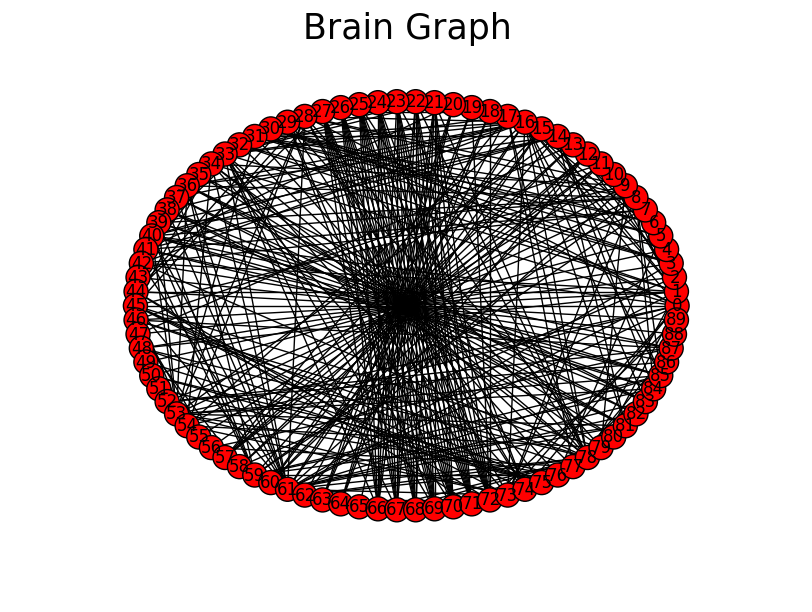
\includegraphics[width=0.45\textwidth]{Figures/brain_graph.png}      

    \rule{35em}{0.5pt}
  \caption[Binarizing via thresholding]{How to build a brain graph : The empirical data matrix derived from fMRI-BOLD technique (on the upper left) is binarized via a threshold value $r=0.55$ and its corresponding adjacency matrix (on the upper right). The black spots represent 1's indicating edges between nodes, whereas the white squares represent 0's implying no edge at all. The adjacency matrix is embedded on human cortex axially (on the lower left) with \textsc{BrainNet Viewer} \citep{XYZ13} and the brain graph derived from the adjacency matrix with \textsc{NETWORKX} (on the lower right).}
  \label{fig:Binarizing via thresholding}
 %\end{tabular}	
\end{figure}

Figure 2.1 illustrates the exemplary construction of a brain graph from the FCM. All correlation values among the cortical and sub-cortical regions in the empirical fMRI-BOLD data lie between 0 and 1. 3D axial cortex visualization represents only the existing edges with black edges among the nodes. The adjacency matrix (AM) is filled out only with 1's and 0's indicating functionally connected and unconnected nodes, whose correlated BOLD activity is equal to or greater than $r=0.55$. The algorithm \textsc{Networkx} builds the corresponding graph of an adjacency matrix. The AM obtained from an ACM would look similar, but would represent the probability of two nodes to be anatomically connected above a predefined threshold $p$. 

The following sections will cover randomization methods reshuffling the brain graphs and introduce some of the topological concepts characterizing brain graphs as well as random networks.



\section{Randomization Methods}





\subsection{Erd\H{o}s-R\'{e}nyi Type Randomization}

Given a total number of nodes $N$, Paul Erd\H{o}s and Alfr\'{e}d R\'{e}nyi produced an undirected graph $G(N,P)$, in which the presence of any edge between two nodes is assigned a probability $P$. 
The average total number of edges $L$ in an  Erd\H{o}s-R\'{e}nyi type random graph is $\binom {N} {2}P$, with a binomial distribution for the number of edges per node.

New randomization techniques arise through modifying the Erd\H{o}s-R\'{e}nyi method, e.g. given $N$ and $L$, a graph $G(N,L)$ can be picked uniformly random out of set of all potential graphs having $N$ nodes and $L$ edges. The probability for a graph to be picked among all the others is $\frac{L}{\binom {N}{2}}  $. One can study the various aspects of $G(N,P)$ and $G(N,L)$ even more detailed, but for the sake of simplicity, Erd\H{o}s-R\'{e}nyi model will not discussed further here.

\begin{figure}[htbp]
 %\begin{tabular}{cc}
  \centering
	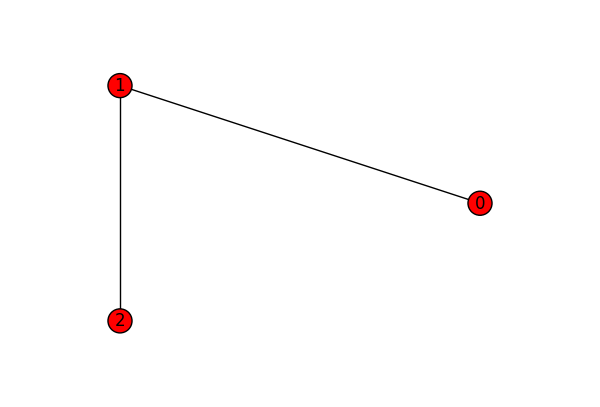
\includegraphics[width=0.30\textwidth, height=40mm]{Figures/f1.png}  
	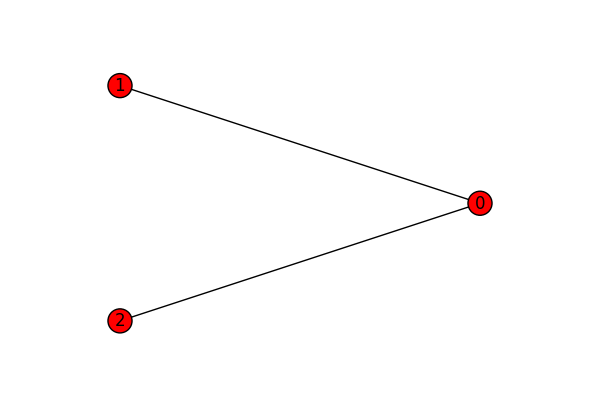
\includegraphics[width=0.30\textwidth, height=40mm]{Figures/f2.png} 
    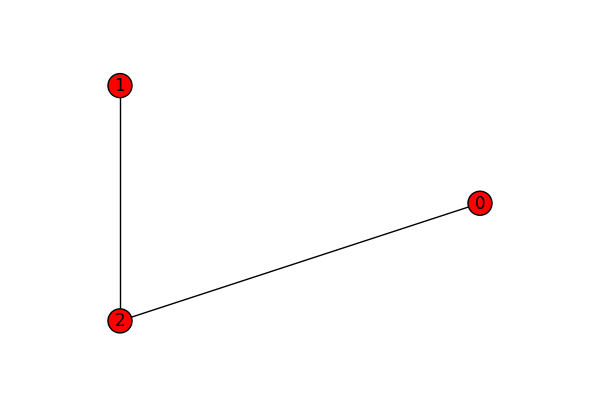
\includegraphics[width=0.30\textwidth, height=40mm]{Figures/f3.png}

    \rule{35em}{0.5pt}
  \caption[Erdos-Renyi Example]{An illustration of the set of all $G(N,L)$ type random graphs with $N=3$ and $L=2$.}
  \label{fig:Erdos-Renyi Example}
 %\end{tabular}	
\end{figure}

Figure 2.2 illustrates all possible graphs having 3 nodes and 2 edges. One of those 3 simple graph is chosen uniformly random for the $G(N,L)$ randomization type, so that each graph is chosen with probability $P=\dfrac{1}{3}$.  

The $G(N,L)$ type randomization is the first method used to derive random graphs from the adjacency matrices of FCM and ACM in this project. Both matrices have $N=90$ nodes, however $L$ changes for each brain graph according to the applied threshold level and therefore is always recalculated. 

\subsection{Double-Edge-Swap Type Randomization}

The \textit{degree} $k_i$ of a node $i$ is defined as the number of edges connected to that node. The double-edge-swap method manipulates a given graph by swapping two existing edges among four nodes, while keeping the node degrees fixed. 


\begin{figure}[htbp]
 %\begin{tabular}{cc}
  \centering
	\includegraphics[width=0.32\textwidth, height=50mm]{Figures/G1_swap.eps}  
    \includegraphics[width=0.32\textwidth, height=50mm]{Figures/G2_swap.eps}  
	\includegraphics[width=0.32\textwidth, height=50mm]{Figures/G3_swap.eps} 
    \rule{35em}{0.5pt}
  \caption[Double-Edge-Swap Example]{Swapping edges between 2 paired nodes}
  \label{fig:Double-Edge-Swap Example}
 %\end{tabular}	
\end{figure}

Figure 2.3 illustrates randomly chosen double edges in a sample graph to be swapped. After the existing edges are removed, the new pair of nodes are rewired. The degree of each node is the same before and after swapping; degrees of nodes $k_1 = 1$, $k_2=1$, $k_3=1$, $k_4=1$ are all fixed in each graph. Although the randomly constructed graphs with the double-edge-swap method are expected to have same degrees, the latter is not a unique property identifying a graph.

The \textit{degree distribution} is the probability distribution of node degrees over the whole graph. Conservation of each $k_i$ preserves the degree distribution, however, preserving degree distribution does not guarantee to fix $k_i$ values. We will discover in the next section how to preserve degree distribution by altering node degrees.

\subsection{Preserved-Degree-Distribution Type Randomization}

The preserved-degree-distribution method randomizes a given network by adding-removing or rewiring its edges randomly while recovering its degree distribution $P(k)$. The idea is to reassign edge indices in the graph, meaning that the degree of individual nodes may change. P(k) is defined with the following equation,

\begin{equation}
P(k) = \sum_{k' \geq k} p(k')
\end{equation}

where $p(k')$ is the probability of a node to have degree number $k'$ \citep{BAR99a}.


\begin{figure}[htbp]
 %\begin{tabular}{cc}
  \centering
	\includegraphics[width=0.45\textwidth, height=60mm]{Figures/G_degree_dist_1.eps}  
	\includegraphics[width=0.45\textwidth, height=60mm]{Figures/G_degree_dist_2.eps}    
    \rule{35em}{0.5pt}
  \caption[Degree Distribution 2D Example]{Reconstruction of a given graph (on the left) with degree-distribution-preservation model (on the right). $k_i=\{3,1,1,1\}$ in the original graph and $k_{i}=\{1,0,1,3,1\}$ in the randomized graph. }
  \label{fig:Degree Distribution Example}
 %\end{tabular}	
\end{figure}

The algorithm is thought to add-remove new nodes to a given graph while preserving $P(k)$ as shown in Figure 2.6. However, we randomize our brain graph with a conserved total number of nodes $N$ as well as $P(k)$. The figure is given only for a better visualization in order to distinguish preserved-degree-distribution randomization method and configuration model randomization, which will be introduced in the next section.

\begin{figure}[htbp]
 %\begin{tabular}{cc}
  \centering
	\includegraphics[width=\textwidth]{Figures/G_degree_dist.eps}  
    \rule{35em}{0.5pt}
  \caption[Degree Distribution 3D Example]{Heat maps for degree distributions of the brain graph obtained from FCM (on the left), and of the randomized graph with preserved-degree-distribution tool (on the right). Colorbars are in logarithmic scale with lower and upper limits : $[\log_{10} {10}^0 , \,  \log_{10} {10}^1]$}
  \label{fig:Degree Distribution 3D Example}
 %\end{tabular}	
\end{figure}

$P(k)$ is a global topological measure for a network, it can be illustrated over all nodes in the whole graph as in Figure 2.7. Node indexes are labeled on $x$ axis on heat maps, threshold $r$ values for adjacency matrices are given on $y$ axis. The preserved-degree-distribution method generates successfully a random graph with the same $P(k)$ as in the brain graph. 


\subsection{Configuration Model Randomization}

The \textit{degree sequence} of a graph is either its ascending or descending sequence of node degrees. The configuration model generates a random graph with a given degree sequence. The direct implementation of this model is to assign edges to the nodes randomly until the desired degree sequence is matched. The resultant random graph is expected to be a node-index-shuffled version of the original graph. However, these algorithms are non-trivial due to the occurrence of self-loops (node is connected to itself) and parallel edges (multiple edges connecting two nodes), which are both undesirable graph properties in this project. 

\begin{figure}[htbp]
 %\begin{tabular}{cc}
  \centering
	\includegraphics[width=0.45\textwidth, height=60mm]{Figures/G_config_1.eps}  
	\includegraphics[width=0.45\textwidth, height=60mm]{Figures/G_config_2.eps} 
    \rule{35em}{0.5pt}
    \caption[Degree Sequence Definition]{The degrees of the nodes in the original graph (on the left): $k_0 = 2$, $k_1 =1$, $k_2=2$, $k_3=3$ and that of the randomized graph (on the right) : $k_0 = 3$, $k_1 =2$, $k_2=1$, $k_3=2$. The degree sequence in non-increasing order in both graphs : $\{3,\,2,\,2,\,1\}$}
  \label{fig:Degree Sequence Definition}
 %\end{tabular}	
\end{figure}

Figure 2.8 points out the relevance of the degree sequence to the node degrees. Moreover, one should not confuse degree distribution and degree sequence.   

The configuration model variant used here is the expected-degree-graph method, which excludes self-loops and parallel edges. This algorithm receives the list of the expected degree sequence as an input $(k_u, k_v, k_m, k_l, ...)$, and assigns edges between nodes with a predefined probability $P_{uv}=\dfrac{k_u k_w}{\sum_{i}k_i}$. This method does not guarantee to construct graphs with exactly the same given degree sequence but with the closest possible sequence.  



 
\subsection{Partial Randomization}
 
The partial randomization method  reconstructs a graph (say A) with partial rewirings with respect to a second graph (say B) while keeping the degree distribution the same as in A. The analogy of this algorithm is to perform rewirings in the adjacency matrix of A, while avoiding any edge generation which already exist in the B. In other words, the choice of edges to be performed rewirings in A is limited with respect to the B. 

In this project, the functional connectivity (FC) adjacency matrix is partially rewired with respect to the anatomical connectivity (AC) adjacency matrix.  This means doing such rewirings among the nodes in FCM only if these nodes are not structurally connected in the brain with probability above a given value. The same procedure is done to randomize AC adjacency matrix partially with respect to FC adjacency matrix.  This time nodes in ACM can be linked only if they are not functionally correlated above a given threshold.   

\begin{figure}[htbp]
 %\begin{tabular}{cc}
  \centering
	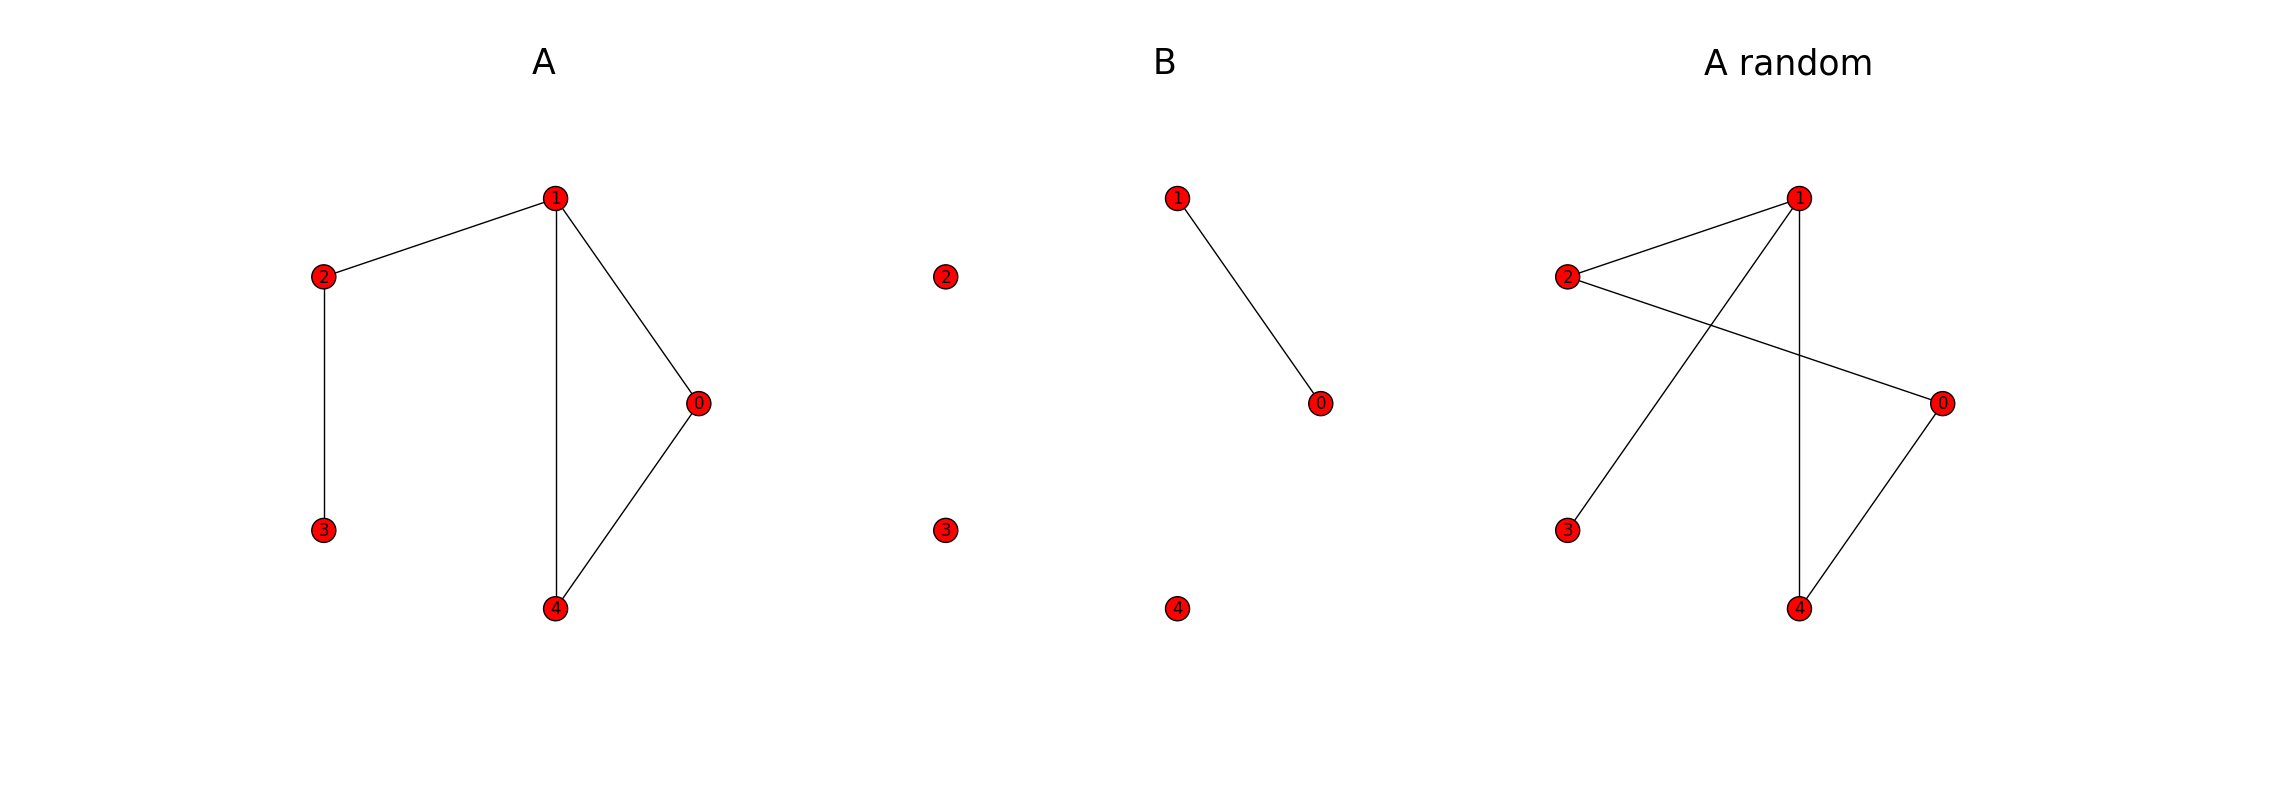
\includegraphics[width=\textwidth, height=55mm]{Figures/p1.png}  
    \rule{35em}{0.5pt}
    \caption[Partial Randomization Example]{Graph A is performed a partial randomization with respect to graph B. While the partial randomization tool rewires edges in A, it avoids creating such edges that exist in B.}
  \label{fig:Partial Randomization Example}
 %\end{tabular}	
\end{figure}

Representative graphs $A$ and $B$ in Figure 2.9 can be thought as FCM and ACM, respectively. In this case, $A \,\, random$ is the partially randomized graph of FCM with respect to ACM.


The brain graph and randomly generated graphs will be identified in terms of their topological properties in the following sections. For simplicity the abbreviations are introduced in the table below. 

\begin{table}[h]
\begin{center}
\caption[Abbreviations]{Abbreviations for the brain graph and the randomly constructed graphs. }
\begin{tabular}{ l | c | r }
  Abbreviation & Description & method \\
  \hline  \hline                     
  R0 & the brain graph						  & \textsc{networkx} \\ \hline
  Ra & Erd\H{o}s-R\'{e}nyi, G(N,L)            & \textsc{networkx} \\ \hline
  Rd & double-edge-swap            			  & \textsc{networkx} \\ \hline
  Rh & preserved-degree-distribution		  & \textsc{BCT} 	 \\ \hline  
  Rg & configuration model       			  & \textsc{networkx} \\ \hline
  Rk & partial randomization            	  & \textsc{BCT} 	 \\ \hline  
  \hline  
\end{tabular}
\label{table:Abbreviations}
\end{center}
\end{table}	

\section{Network Characterizations}

\subsection{Network Density}
The \textit{average degree} $\langle k \rangle$ of a network is proportional to the ratio of total number of edges $L$ to total number of nodes $N$ in a graph, 

\begin{equation}
\langle k \rangle = \frac{2L}{N}.
\end{equation}

It should be noted that in order to not count each edge twice, the total number of edges is divided by $N/2$ instead of $N$. The \textit{density} $D$ of a network is a scaled version of average degree measurement. It is formulated as the ratio between $L$ and maximum number of possible edges ${N \choose 2}$,

\begin{equation}
D = \frac{2L}{N(N-1)}.
\end{equation}	

The measure of network density can be referred to as the total \textit{wiring cost} of the network \citep{RUB10}. The degree, average degree and network density are key scalar measures to characterize the topology of a network. There is for instance clinical evidence that reductions in nodal degree are associated with greater severity of local amyloid deposition in patients with Alzheimer's disease \citep{XYZ2009}. 

\begin{figure}[htbp]
 %\begin{tabular}{cc}
  \centering
	\includegraphics[width=0.48\textwidth, height=55mm]{Figures/Network_Density_Fnc.eps}
	\includegraphics[width=0.48\textwidth, height=55mm]{Figures/Network_Density_Stru.eps}  
    \rule{35em}{0.5pt}
    \caption[Network Density]{Network density of the brain graphs and random graphs of FCM (on the left) and ACM (on the right). The abbreviations are chosen as described in Table 1.}
  \label{fig:Network Density}
 %\end{tabular}	
\end{figure}


The network density $D$ can be considered a probability for all graphs in corresponding threshold $r$ and $p$ ranges. The random networks are built in such ways that they have the same number of nodes and almost the same $D$ as in the brain graphs. However, the $D$ is not a unique metric identifying a network.

All networks for FCM and ACM are densely connected for low $r$ and $p$. For the brain graph and randomized graphs of FCM, $D$ decreases sigmoidally with $r$. In comparison, $D$ decreases slower with $p$ for ACM graphs. It should be noted that all graphs have almost the same $D$ values. 

Functional networks are likely to be denser than anatomical networks, as they will typically contain numerous connections between anatomically unconnected regions \citep{DAM09}. 

\subsection{Average Clustering Coefficient}
    
The \textit{average clustering coefficient} $C$ of a network is calculated through individual clustering coefficients $C_i$ of single nodes,

\begin{equation}
C = \frac{1}{n} \sum\limits_{i\epsilon N}C_i = \frac{1}{n}\sum\limits_{i\epsilon N} \frac{2t_i}{k_i(k_i -1)} .
\end{equation} 

where $t_i$ is the number of triangles around node $i$ and $k_i$ is the degree of node $i$ \citep{WAT98}. The clustering coefficient is a measure of segregation, that is the ability for specialized processing to occur within densely interconnected groups of brain regions \citep{RUB10}. It reveals how the individual nodes in a graph cluster together; how many neighbors of a node are neighbors of each other. 

\begin{figure}[htbp]
 %\begin{tabular}{cc}
  \centering
	\includegraphics[width=0.48\textwidth, height=55mm]{Figures/Clustering_Coefficient_Fnc.eps}
	\includegraphics[width=0.48\textwidth, height=55mm]{Figures/Clustering_Coefficient_Stru.eps} 
    \rule{35em}{0.5pt}
    \caption[Clustering Coefficient]{Average clustering coefficient of the brain graphs and random graphs of FCM (on the left) and ACM (on the left). }
  \label{fig:Clustering Coefficient}
 %\end{tabular}	
\end{figure}

The clustering coefficient $C_i$ of a node $i$ is a measure of local connectivity and is highly correlated with the local efficiency of the information transfer \citep{LAT01}. The $C_i$ is formulated as the ratio of $t_i$ over all possible edges of the node $i$; ${k_i \choose 2} $. The average clustering coefficient $C$ is a normalized version of $C_i$ for the whole network, yielding now a global property. All $C$ values are between 0 and 1. Figure 2.7 shows that at lower binarization thresholds, nodes tend to cluster more due to higher number of existing edges. The empirically obtained brain networks of FCM and ACM have the highest $C$ compared to random graphs. The local information transfer seems to be more efficient in the brain graphs.  The randomized graphs of ACM $Ra$, $Rd$, $Rh$ and $Rk$ share more nodes with lower degrees compared to $R0$.

\subsection{Transitivity}

Transitivity is a similar measure to the clustering coefficient, and also quantifies segregation in the network. It is defined as \citep{NEW03}
	
\begin{equation}
 T = \frac{\sum\limits_{i \epsilon N} 2 t_i}{\sum\limits_{i \epsilon N}k_i (k_i - 1)} .
\end{equation}	

If a node has links to two other nodes, transitivity inquires whether those two other nodes are also connected to each other. It asks, what percentage of triangles in the network is closed. Transitivity resembles clustering coefficient, however, it is defined only for the whole network rather than single nodes. 

\begin{figure}[htbp]
 %\begin{tabular}{cc}
  \centering
	\includegraphics[width=0.48\textwidth, height=55mm]{Figures/Transitivity_Fnc.eps}
	\includegraphics[width=0.48\textwidth, height=55mm]{Figures/Transitivity_Stru.eps} 
    \rule{35em}{0.5pt}
    \caption[Transitivity]{Transitivity of the brain graphs and random graphs of FCM (on the left) and ACM (on the left). }
  \label{fig:Transitivity}
 %\end{tabular}	
\end{figure}


The degree of transitivity is one of the fundamental differences between real world networks and random networks \citep{NEW10}. This difference is more pronounced than the clustering difference between brain graphs and random graphs (see Figures 2.7 and 2.8). $T$ is more effected with $P(k)$ of a network, the more nodes with lower degrees, the higher the $T$ is. ACM related graphs tend to have lower $p(k')$ values distributed among many nodes, whereas FCM related graphs have higher $p(k')$ values distributed among less nodes. This holds even for $R0$ and $Rh$ graphs of FCM in Figure 2.12, that their $P(k)$ is reflected in higher $T$ (see Appendix).



\section{FitzHugh-Nagumo Model for Neuronal Activity Simulation}

An fMRI-BOLD experiment reveals the correlation coefficients between timeseries of BOLD activity among pre-defined brain regions. The empirical functional connectivity matrix (FCM) derived from fMRI-BOLD technique in this project reflects those coefficients among $N=90$ AAL regions at the resting state of human brain, i.e. no stimulus driving approach is introduced to the subject. Despite lack of any stimulus, the observed fMRI-BOLD signal in the mammalian brain is highly structural and robust at low frequency fluctuations ($<$0.1 Hz) \citep{BIS95, DAM06, VIN07a}. However, the underlying reason of these well organized spatio-temporal dynamics has not yet been completely resolved. The existing models of resting-brain dynamics hypothize that functional interactions result from a complex interplay between intrinsic brain dynamics and anatomical connections \citep{RUB09}. This section proposes a modeling approach for the ongoing neuronal activity at brain's resting state, i.e. how  underlying correlated behavior among distant cortical brain regions arise \citep{VUK13}. Once the model is fulfilled with bio-physically plausible parameter ranges with the help of previous studies, the timeseries of nodes in brain graphs will be extracted by means of model simulations as well as in randomly constructed networks. 

The theoretical model of choice for the neuronal activity is FitzHugh-Nagumo (FHN) systems describing physiological states of nerve membrane potential \citep{FIT61, NAG62}. FHN model will be used to represent the neuronal activity of a nerve cell population, in other words, an AAL node in this project. Local dynamics of a single node will then be globalized in the whole brain network via mutual time delayed interactions among nodes. Here, time delay $\delta \tau_{ij}$ is assumed to arise from a limited signal propagation velocity $v$ between nodes $i$ and $j$, furthermore, time delayed interactions are scaled with a coupling strength $c$ \citep{GHO08, GHO08a, DEC09}. Another important parameter for FHN simulations is threshold $r$ or probability $p$ values used to extract adjacency matrices from FCM and ACM. The first objective is to investigate such plausible $c$, $v$, and $r$ or $p$ ranges at which our simulated neuronal activity of brain graphs are similar to the empirical fMRI-BOLD data. 

FHN model will also be applied on randomly constructed graphs described in the previous section. The second objective is to identify such regions in the explored parameter space for which the simulated timeseries of the empirically obtained networks are distinguishable than that of randomly constructed graphs. The effects of $c$, $v$, $r$ or $p$ as well as network characteristics of graphs will be taken into consideration. At the end, it is aimed to gain further insight into the key features of anatomical brain structures by comparing to randomized networks.  
 
The FHN model is designed to reflect the neuronal activity as simulated timeseries, it is not corresponding the BOLD activity. The comparison of simulated BOLD activity to the fMRI-BOLD signal would be ahead of timeseries comparison approach. The last objective of FHN model is the following: the simulated neuronal activity will be finally used to infer the BOLD signal via the Baloon-Windkessel hemodynamic model in the last section \citep{FRI00}. 

Subsections will describe set of non-linear differential equations for the FHN local dynamics and carry out a stability analysis. Dynamics of a single node will then be globalized via mutual couplings with a second node and the effect of time delay interactions will be demonstrated. The last part will embed complete FHN simulation to a simple graph and the first exemplary timeseries of a node will be illustrated. 





\subsection{FHN Model Local Dynamics}

This section aims to demonstrate local dynamics of a brain node with FHN model. Here, the node is assumed to be isolated, meaning that it is not connected to any other node at all in the brain. FHN model has an activator variable $x$ and an inhibitor variable $y$, their time evolution is represented with the same implementation as in \citep{GHO08, GHO08a} in following non-linear differential equations,
\begin{subequations}
\begin{align}\dot{x} = \tau (y + \gamma x - \frac{x^3}{3})  \label{eqn: frobenius 1}\\  \dot{y} = -\frac{1}{\tau} (x - \alpha + b y - I ) \label{eqn: frobenius 2}   \end{align} 
\end{subequations}
where $\tau$ denotes the time constant accelerating $x$, $I$ is the external stimulus parameter and $\gamma$, $\alpha$, $b$ are other system parameters. $x$ and $y$ are considered to be counteracting variables capturing membranous potential alterations on a neuronal population around $10^9$ cells. Non of the activator or the inhibitor variables includes any coupling parameter for the described local activity and additionally $I$ is chosen to be 0 \citep{GHO08}.

The \textit{fixed point} $(x_f, y_f)$ of the system is defined such that there is no change in variables over time $\dot{y} =\dot{x} = 0 $. The fixed point condition substituted back into equations (2.6a) abd (2.b6) yields set of $nullcline$ equations, 
\begin{subequations}
\begin{align}  y = \frac{x^3}{3} - \gamma x
              \label{eqn: frobenius 3}\\  
               x = \alpha - b y
               \label{eqn: frobenius 4}   \end{align} 
\end{subequations}
where equation (2.7a) will be called as $y-nullcline$ and (2.7b) as $x-nullcline$ from now on. The stability analysis is performed by calculating eigenvalues of the \textit{Jacobian Matrix}, \textbf{J} at the intersection of nullclines, $(x_f, y_f)$. The  linearization of equations (2.6a) and (2.6b) helps to find  \textbf{J} straightforward,
\begin{equation}
%
    \begin{pmatrix}
        \frac{dx}{dt} \\ \frac{dy}{dt}
     \end{pmatrix} = \begin{pmatrix}
        \tau(\gamma - x_f^2) & \tau \\
        -\frac{1}{\tau}     & -\frac{b}{\tau}
     \end{pmatrix}
    \begin{pmatrix}
        x \\
        y
    \end{pmatrix}
%
\end{equation}
where,
\begin{subequations}
\begin{align} \textbf{J} = \begin{pmatrix} \tau(\gamma - x_f^2) & \tau \\ -\frac{1}{\tau}     & -\frac{b}{\tau}   \end{pmatrix}
              \label{eqn: frobenius 5}\\  
 \det \textbf{J} =  b(x_f^2 - \gamma) +1
               \label{eqn: frobenius 6} \\   
\mathrm{tr} \textbf{J} =  \frac{1}{\tau}(\tau^2( \gamma - x_f^2 ) -b)
               \label{eqn: frobenius 7}                 
               \end{align} 
\end{subequations}
Eigenvalues of \textbf{J} are calculated as the following,
\begin{subequations}
\begin{align} \det \begin{pmatrix} \textbf{J} - \lambda \textbf{I} \end{pmatrix} = 0
              \label{eqn: frobenius 8}\\  
 \lambda^2 - \lambda \mathrm{tr} \textbf{J} + \det \textbf{J} = 0
               \label{eqn: frobenius 9} \\
\lambda_{1,2} = \dfrac{\mathrm{tr} \textbf{J} \pm \sqrt{\mathrm{tr} ^1 \textbf{J}} -4 \det \textbf{J} }{2}               
                \label{eqn: frobenius 10} \\    
\lambda_{1,2} = \dfrac{\tau^2(\gamma - x_f^2)-b \pm \sqrt{(\tau^2(x_f^2-\gamma)-b)^2 - 4 \tau^2 }}{2 \tau}
               \label{eqn: frobenius 11}                 
               \end{align} 
\end{subequations}

Parameters in FHN model are tuned so that solutions would render a damped oscillatory behavior for each node locally;  $\alpha = 0.85$, $b=0.2$, $\gamma=1.0$ and $\tau=1.25$ \citep{VUK13}. The solution of the condition $\dot{y}=\dot{x}=0$ gives coordinates of $(x_f, \, y_f) = (0.98 \, , -0.67 )$, which is calculated numerically here. All parameters plugged in eigenvalue equation (2.10d) results in $\lambda_1 = -0.056 + 0.996 i$ and $\lambda_2 = -0.056 - 0.996 i$. Since real parts of both eigenvalues stand below zero, the fixed point is said to be \textit{stable}. $\lambda_1$ and $\lambda_2$ are complex conjugate pairs, the fixed point can be alternatively called as a \textit{stable focus}. Variables $x$ and $y$ are expected to relax onto the fixed point over time.  

\begin{figure}[htbp]
  \centering
	\includegraphics[width=\textwidth]{Figures/FHN_local.eps}
 
    \rule{35em}{0.5pt}
    \caption[FHN Local]{Local dynamics of an isolated node: time evolution of $x$ and  $y$ (on the left) and nullclines on state space together with $x(t),y(t)$ (on the right). The fixed point $(x_f, \, y_f) = (0.98 \, , -0.67 )$ is drawn with a black dot at the intersection of nullclines and initial point $(x_0, y_0)$ is illustrated with a red dot.  }
  \label{fig:FHN Local}	
\end{figure}

The time evolution of $x$ and $y$ resembles damped oscillations at the beginning. Following to a rapid excitation and inhibition, both variables converge to the fixed point. State space illustrates this relaxation over nullclines, a clockwise trajectory starting from a randomly chosen $(x_0, y_0)$ and felling on $(x_f, y_f)$ with smaller and smaller amplitude oscillations. The system is in quiescent state, but can also be said to be at the onset of instability. The scale of change in $x$  is more pronounced than $y$ due to $\tau$ proportionality in the definition of $\dot{x}$ in FHN model.  
 
\subsection{Noise Effect}

The local dynamics of a node can be extended with an additional noise factor, 
\begin{subequations}
\begin{align}\dot{x} = \tau (y + \gamma x - \frac{x^3}{3}) + Dn_x  \label{eqn: frobenius 12}\\  \dot{y} = -\frac{1}{\tau} (x - \alpha + b y - I ) + Dn_y \label{eqn: frobenius 13}   \end{align} 
\end{subequations}
where $D$ is the noise strength, $n_x$ and $n_y$ represent Gaussian white noises. Neither coordinates of the fixed point or eigenvalues are affected due to the noise factor. However, dynamics of the system is forced to go under a change such that the stability will be lost. 

\begin{figure}[htbp]
  \centering
	\includegraphics[width=\textwidth]{Figures/FHN_noise.eps}
 
    \rule{35em}{0.5pt}
    \caption[FHN Noise]{Local dynamics of two variables $x$ and  $y$ with same parameters as previously stated, an additional Gaussian white noise with strength $D=0.05$ is added. The fixed point $(x_f, \, y_f) = (0.98 \, , -0.67 )$ is drawn with a black dot in state space where two nullclines intersect.   }
  \label{fig:FHN Noise}	
\end{figure}

The noise drives sub-threshold oscillations as realized in the time evolution of activator and inhibitor. It prevents $x$ and $y$ variables from relaxing on the fixed point, instead, they fluctuate around it. This dynamics remarks the onset of instability, and it is called "type II excitation" in terms of neuronal dynamics. 


\subsection{Global Dynamics}

This section demonstrates the effect of mutual coupling between two exemplary nodes with FHN model. Now, we consider two nodes connected to each other, either functionally or structurally as in FCM or in ACM. The effect of this connection is captured theoretically with a global coupling term and time delayed interactions, 

\begin{subequations}
 \begin{align}\dot{x_1} = \tau (y_1 + \gamma x_1 - \frac{x^3}{3}) + C [x_2(t-\tau_{12})] +Dn_{x1} \label{eqn: frobenius 14}\\  \dot{y_1} = -\frac{1}{\tau} (x_1 - \alpha + b y_1 - I )+ Dn_{y1} \label{eqn: frobenius 15} \\ \dot{x_2} = \tau (y_2 + \gamma x_2 - \frac{x_2^3}{3}) + C [x_1(t-\tau_{21})] + Dn_{x2} \label{eqn: frobenius 16} \\  \dot{y_2} = -\frac{1}{\tau} (x_2 - \alpha + b y_2 - I ) + Dn_{y2}\end{align} 
\end{subequations}
 
where $C$ is the coupling strength, subindices 1 and 2 stand for corresponding nodes, $\tau_{12}$ and $\tau_{21}$ are time delays required for coupled node interactions and $D$ is the Gaussian white noise strength. For simplicity, the global dynamics are illustrated with same local parameters as before, while time delays are taken to be homogeneous, $\tau_{12}=\tau_{21}=0.5$.

\begin{figure}[htbp]
  \centering
	\includegraphics[width=\textwidth]{Figures/FHN_global.eps}
 
    \rule{35em}{0.5pt}
    \caption[FHN Global]{Global dynamics of two nodes with variables $x_1,y_1$ and  $x_2,y_2$. The fixed point is the same for both systems $(x_f, \, y_f) = (0.98 \, , -0.67 )$, it is drawn with a black dot at the intersection of nullclines in state space.}
  \label{fig:FHN Global}	
\end{figure}

The mutual coupling between nodes pushes both systems $(x_1,y_1)$ and $(x_2,y_2)$ to be oscillatory with visibly larger amplitudes in comparison to local dynamics and noise effect in previous figures. The system does not fall on to the fixed point anymore, indicating loss of the stability. 

\subsection{FHN Time Series}

After introducing the local and global dynamical models of nodes, the final version of FHN model to be simulated as the neuronal activity in the complete brain graph or random network is denoted with the following notation \citep{VUK13},  
 
\begin{subequations}
 \begin{align}\dot{x_i} = \tau (y_i + \gamma x_i - \frac{x_i^3}{3}) -c \sum_{j=1}^N a_{ij}x_j(t - \Delta t_{ij}) +Dn_x \label{eqn: frobenius 17}\\  \dot{y_i} = -\frac{1}{\tau} (x_i - \alpha + b y_i - I ) +Dn_y \label{eqn: frobenius 18}   \end{align} 
\end{subequations}

where the index $i$ represents any node among $N=90$ AAL regions, $c$ is coupling strength, $a_{ij}$ is corresponding connectivity unit between nodes $i$ and $j$ in adjacency matrix. This is the crucial link between network analysis part and FHN section. If nodes are connected in a given network, then $a_{ij}=1$, otherwise $a_{ij}=0$. $\Delta t_{ij}$ is the time delay factor arising from finite signal propagation velocity $v$ among nodes. $\Delta t_{ij}$ is calculated as $\Delta t_{ij}=\frac{d_{ij}}{\nu}$ \citep{GHO08, GHO08a, DEC09}, where $d_{ij}$ is the matrix of Euclidean distances between centers of brain regions from which BOLD time series are extracted \citep{KAI06}. The external stimulus is again set to zero $I=0$. The noise ($n_x$, $n_y$) factors are Gaussian white noise distributions, the strength of noise is $D=0.05$, large noise.
 
\begin{figure}[htbp]
  \centering
	\includegraphics[width=\textwidth]{Figures/FHN_graph.eps}
 
    \rule{35em}{0.5pt}
    \caption[FHN Graph]{Two sample graphs to be simulated with FHN model, the upper-most node, say node 1 is not connected at all in first graph (on the left) and connected by 3 edges in second graph (on the right).  }
  \label{fig:FHN Graph}	
\end{figure}


\begin{figure}[htbp]
  \centering
	\includegraphics[width=\textwidth]{Figures/FHN_time_1.eps}
 	\includegraphics[width=\textwidth]{Figures/FHN_time_2.eps}
    \rule{35em}{0.5pt}
    \caption[FHN Time Series]{Analogous time series of node 1 chosen from graphs illustrated in previous figure. Timeseries at top is of the unconnected node, at down is of 3-edge connected node. All parameters besides $d_{ij}$ matrix are chosen to be biologically plausible. An unrealistic $d_{ij}$ is filled out for corresponding sample graphs in previous figure.  }
  \label{fig:FHN Time Series}	
\end{figure}

The time delay coupled set of ordinary differential equations is solved numerically with \textsc{PYTHON}-module \textsc{PYDELAY}-algorithm based on Bogacki-Sampine method \citep{FLU09a, BOG89}. 


FHN timeseries of node 1, having no edge connections in first graph, is oscillatory, but the scale of oscillations seem to be small. Its dynamical view is in agreement with FHN local dynamics with noise effect. However, when node 1 is connected to 3 other nodes in second graph, then large scaled oscillatory patterns of its activator and inhibitor variables can be observed as a consequence of global coupling terms. 

This section proposed to describe the chosen theoretical model for the neuronal activity. The next step is to study the introduced neuronal dynamics on empirically derived and randomly constructed graphs. $N=90$ nodes  in any given network will be simulated with the complete FHN timseries notation for 7.5 minutes. Then, Pearson correlation coefficients between simulated timeseries of node pairs will be calculated for one graph. A $90X90$ correlation matrix will raise for each FHN simulated network.

FHN model is involved in crucial steps in this Master's project: parameter analysis, distinguishing brain graphs and random graphs and finally extracting BOLD activity. Simulations on brain graphs obtained from FCM and ACM matrices will be compared to the original fMRI-BOLD data in parameter spaces by tuning three parameters in bio-physically plausible ranges: coupling strength $c$ and velocity $v$ as well as a threshold $r$ or probability $p$ value, which is used while constructing adjacency matrices $a_{ij}$ of given graphs. Simulations on random graphs will be used to identify regions in the explored parameter space for which the empirical data differ from that of the random graphs. Not only the effect of tuned parameters $c$, $v$ and $r$ or $p$, but also the contribution of topological measurements of graphs will be taken into account. At the end, FHN timeseries of brain graphs will be simulated further with another theoretical model to capture the BOLD signal, which will be introduced in the next session.   



\section{Balloon-Windkessel Model for BOLD Activity Simulation} 

Blood oxygen level dependent (BOLD) effect is one of the underlying contrast mechanisms of fMRI to map brain activity at resting state. BOLD signal is thought to arise from interactions between neuronal activity and regional changes in the surrounding of those active neurons such as blood volume, blood flow and  oxygenation level in capillaries. When neuronal activity increases, the blood flow in blood vessels surrounding this neuronal region rises, causing a change in relative amounts of deoxygenated and oxygenated forms of Hemoglobin (dHB and Hb). The difference in magnetic properties of dHb (paramagnetic) and Hb (diamagnetic) is the key ingredient to the observed changes in magnetic resonance signal. A better understanding of the resting state BOLD signal is required to better interpret neuronal activity. The previous section proposed already a model for the neuronal activity, FHN model. This section will introduce a hemodynamic process to capture BOLD activity with a mathematical model known as Balloon model \citep{XYZ98}. 

In addition to the variations in magnetic properties of the blood caused by blood flow in vessels, there are other physiological changes during alteration in neuronal activity that affect the temporal dynamics of BOLD signal, i.e. cerebral blood flow (CBF), cerebral blood volume (CBV), cerebral metabolic rate of oxygen consumption (CMR$O_2$). Moreover, the BOLD response is subject dependent: the physiological baseline state of the individual under examination is used to scale BOLD response and this fact brings another difficulty to interpret the BOLD signal, when the baseline state varies \citep{XYZ2013}. The sensitivity of BOLD signal to the variations in vascular and metabolic physiology brings a great complexity to interpret it accurately. The biophysical descriptions of the BOLD signal are still not fully satisfactory for the resting state. 

Changes in the BOLD signal obtained in an fMRI experiment represent an indirect measure of underlying neuronal activity \citep{VUK14}. The modeled neuronal activity can be used to infer the BOLD signal observed in the fMRI data via Baloon-Windkessel hemodynamic process, which mediates between a non-linear timeseries and measured BOLD response \citep{FRI00}. In short, the Baloon-Windkessel model picks an input signal from neuronal activity timeseries and turnouts the BOLD activity timeseries as a function of changes in CBF, CBV, CMR$O_2$. The main input of Baloon-Windkessel model is a neuronal signal in the form of either a spiking rate or a local field potential \citep{SET12}. The neuronal signal in this project will be normalized FHN timeseries of activator variable, which describes the excitatory membrane potential dynamics of a neuronal population.       

The study of Friston et al. shows that it is possible to capture ultra-slow frequency oscillations ($<0.1$) in the hemodynamic process, given a higher frequency neuronal input for event related responses \citep{FRI00}. Here, the same model will be tested for the resting state activity to find out whether it is possible to extract BOLD activity from FHN modeled $N=90$ AAL brain nodes. Each brain graph obtained from FCM and ACM data sets will be embedded into Baloon-Windkessel model, and a new parameter analysis will be carried out while comparing resultant BOLD simulations to the fMRI-BOLD empirical data set.

This section is designed to review the Ballon-Windkessel hemodynamic model by demonstrating its input-state-output description very briefly \citep{FRI00}.    

\subsection{Hemodynamic Model}

\begin{figure}[htbp]
  \centering
	\includegraphics[width=\textwidth]{Figures/BOLD_Hemo.eps}
 	\rule{35em}{0.5pt}
    \caption[Hemodynamic Model]{The hemodynamic model for the BOLD activity illustrated in Friston et al. \citep{FRI00}  }
  \label{fig:Hemodynamic Model}	
\end{figure}


\begin{table}[h]
\begin{center}
\caption[BOLD Abbreviations]{Abbreviations for used in hemodynamic model }
\begin{tabular}{ l | c }
  Abbreviation & Description \\
  \hline  \hline                     
  $u(t)$ &      nonlinear input signal  
\\ \hline

  s & blood flow inducing signal 
\\ \hline
  $\tau_s$ & time constant to describe $\dot{s}$  
\\ \hline  
  $f_{in}$ & cerebral blood inflow      
\\ \hline
 $\tau_f$  & time constant to describe $\dot{f_{in}}$ 
\\ \hline  
 $v$    & CBV    
\\ \hline
 $\tau_0$  & time constant to describe $\dot{v}$    
\\ \hline 
 $\alpha$  & a parameter to describe flow-volume relationship
\\ \hline 

  $f_{out}(v, \alpha)$ & cerebral blood outflow function
\\ \hline
 $E_0$  & resting net $O_2$ extraction rate 
\\ \hline
 $E(f_{in}, E_0)$    & fraction of $O_2$ extracted from $f_{in}$    
\\ \hline
 $q$    &  dHB content in voxel 
\\ \hline
 $y(t)$    &  output BOLD signal          \\
\hline  
  \hline 
 
%  \hline  
\end{tabular}
\label{table:BOLD Abbreviations}
\end{center}
\end{table}	





\begin{subequations}
 \begin{align} \dot{s} = \epsilon u(t)- \frac{s}{\tau_s} - \frac{f_{in} -1 }{\tau_f}  \label{eqn: frobenius 18}\\  \dot{f_{in}} = s
\label{eqn: frobenius 19} \\ \dot{v} = \frac{f_{in}}{\tau_0} - \frac{f_{out}(v, \alpha)}{\tau_0} 
\label{eqn: frobenius 20} \\ \dot{q} = \frac{f_{in} E(f_{in}, E_0)}{\tau_0 E_0}- \frac{f_{out}(v, \alpha)}{\tau_0}  \frac{q}{v}  
\
\end{align} 
\end{subequations}

\begin{subequations}
 \begin{align} f_{out}(v, \alpha) = v^{1/ \alpha}
 \label{eqn: frobenius 21}\\  E(f_{in} , E_0) = 1- (1-E_0)^{1/f_{in}} \
\end{align} 
\end{subequations}




\begin{equation}
y(t)= \lambda (v,q,E_0) = V_0 (k_1(1-q) + k_2(1- \frac{q}{v}) + k_3(1-v)))
\end{equation} 






 
%----------------------------------------------------------------------------------------
 
% Chapter 3

\chapter{Results} % Main chapter title

\label{Chapter3} % For referencing the chapter elsewhere, use \ref{Chapter1} 

\lhead{Chapter 3. \emph{Results}} % This is for the header on each page - perhaps a shortened title

The functional connectivity (FC) map is derived from fMRI-BOLD technique and it reveals the BOLD fluctuation correlations between any two AAL regions. The anatomical connectivity (AC) map is obtained from DW-MRI measurement and it represents the probability of any two AAL region to be connected by nerve fibers. (see Section 2.1 for FCM and ACM, Appendix A for AAL describtions). Both data sets are derived at the resting-state activity of human brain, i.e. in the absence of any stimulation.

The brain graphs are constructed in two category: via binarizing FC at different threshold $r$ values and binarizing AC maps at varying $p$ values (Section 2.2). Several randomization procedures are implemented to generate random networks by manipulating FC and AC related brain graphs (2.3). The network topology of all graphs are characterized by statistical measures (Section 2.4, Appendix B). 

The neuronal activity of of an AAL region is modeled with the FitzHugh-Nagumo model (Section 2.5) \citep{VUK13, GHO08a}. The BOLD activity is then inferred via the Balloon-Windkessel model (Section 2.6) \citep{FRI00}. All brain and random graphs are firstly simulated with FHN model, their extracted time-series are then used to implement the BOLD activity. The research proposals are to investigate \textit{i)} whether the BOLD dynamics of resting-state can be captured through the AC map of brain and \textit{ii)} if the temporal dynamics of brain graph is distinguishable than that of random networks.       

This section categorizes all results in three parts: neuronal activity simulations, BOLD activity simulations and comparison of brain graphs to randomly constructed graphs. In Section 3.1, FHN network model simulated on brain graphs of FC and AC maps are compared to fMRI-BOLD data and DW-MRI data, respectively. In Section 3.2, the Balloon-Windkessel model applied to neuronal time-series based on brain graphs of FC and AC maps are compared to the single empirical brain map, the fMRI-BOLD data. In Section 3.3, random graphs are simulated with FHN model. The last part aims to illustrate whether or not these random networks can be distinguished from brain graphs in terms of the modeled neuronal activity.  



\section{Neuronal Activity Simulations}

\subsection{Functional Brain Graphs Compared to fMRI-BOLD Data}

The adjacency matrices (AM) are constructed via binarizing the fMRI-BOLD data at threshold $r=[0.54, \, 0.66]$, an exemplary illustration is given in Figure 2.3, Section 2.2. An AM obtained from fMRI-BOLD data represents whether or not any pair of AAL nodes is functionally connected above a defined $r$. The automated anatomical labeling (AAL) of all $N=90$ nodes can be reviewed in Table A.1, Appendix A. The brain graph constructed on the AM for given $r$-values are simulated with FHN network model (Section 2.5). 

This section aims to investigate the temporal dynamics of the neuronal activity in human brain by comparing simulated network to the fMRI-BOLD data. The comparisons are carried to parameter spaces of $(r,v)$ and $(r,c)$, where $v$ is the signal propagation velocity and $c$ is the coupling strength \citep{VUK13, GHO08a}.  

Once the FHN simulated time-series of all nodes in a brain graph are extracted, the correlation of simulated neuronal activity between any node pairs $i,j$ is quantified by Pearson's correlation coefficient $\rho_{i,j}$, 

\begin{equation}
\rho_{i,j} = \dfrac{\big \langle u_i(t) u_{j}(t) \big \rangle - \big \langle u_{i}(t) \big \rangle  \big \langle u_{j}(t) \big \rangle}{ \sigma (u_i(t)) \sigma (u_j(t))}
\end{equation}

where $u_i(t)$ denotes the FHN time-series of the corresponding node $i$,  $\sigma$ stands for standard deviation and $\big \langle \cdot \big \rangle$ represents the temporal average. Figure 3.1 demonstrates excitatory FHN dynamics of two pairs of nodes. Simulated neuronal time-series of nodes 45 and 28 are well correlated ($\rho_{45,28}=0.88$, Figure 3.1, top), whereas that of nodes 90 and 87 are poorly correlated ($\rho_{90,87}=0.13$, Figure 3.1, bottom).

\begin{figure}[htbp]
 
  \centering
	 \includegraphics[width=\textwidth]{Figures/cor_FCM_sim_no_best.eps} 
   	 \includegraphics[width=\textwidth]{Figures/cor_FCM_sim_no_worst.eps} 

    \rule{35em}{0.5pt}
  \caption[Neural Activity Node Dynamics, FCM]{Temporal dynamics of highly (top, $\rho_{45,28}=0.88$) and poorly (bottom, $\rho_{90,87}=0.13$) correlated node couples with FHN model. The simulation parameters are $c=0.2$, $v=7$ m/s, $r=0.60$.} 
    \label{fig:Neural Activity Node Dynamics, FCM}
 	
\end{figure} 



All $\rho_{i,j}$ values among any possible pairwise combination of $N=90$ nodes are then used to built a $90\times 90$  matrix, which is referred to as simulated correlation matrix (CM). The fMRI-BOLD data was in fact used to obtain a functional correlation matrix (FCM). (Figure 2.1 , Section 2.1). Figure 3.2 illustrates a simulated CM and the empirical FCM together for a better visualization. Each colored square represents how strong any pair of nodes $i$ and $j$ addressed on $x$- and $y$-axes are correlated in terms of \textit{i)} their temporal dynamics for the simulated CM, \textit{ii)} their BOLD fluctuations for empirical FCM. Colorbars denote $\rho_{i,j}$-values.


\begin{figure}[htbp]
 
  \centering
	 \includegraphics[width=0.49\textwidth]{Figures/cor_FCM_sim.eps} 
   	 \includegraphics[width=0.49\textwidth]{Figures/cor_FCM_exp.eps} 

    \rule{35em}{0.5pt}
  \caption[High correlated FHN simulation, FCM]{ Simulated CM obtained from FHN network simulations (left) and empirical FCM (right). The parameters of CM are $c=0.2$, $v=7$ m/s, $r=0.60$, overall correlation between two matrices is $\rho_{e,s} = 0.43$}
      \label{fig:High correlated FHN simulation, FCM}
 	
\end{figure}  



In order to compare the modeling approach to the empirical result, both correlation matrices are compared statistically with Pearson's correlation coefficient, the same linear pairwise correlation method again. All correlation values $\rho_{e,s}$ between empirical $e$ and simulated $s$ data matrices are placed on the parameter spaces. Here, the parameter spaces are designed over $(r,v)$ and $(r,c)$ as seen in Figure 3.3. The purpose is to explore the most promising values for three tuning parameters : $r$, which defines the topology of AM, the coupling strength $c$ and signal propagation velocity $v$, which are parameters of the FHN model as explained in Section 2.5.  Each color coded square in Figure 3.3 corresponds to one $\rho_{e,s}$ value. Hot colors represent high correlation between simulated and empirical data, 0 means no correlation at all and cold colors below zero points out anti-correlations.


A correlation value close to 1 in FCM indicates that the quantified functional activities of corresponding nodes in the right and left hemisphere highly resemble each other, see subdiagonals in Figure 3.2 (right). The AAL regions tend to be correlated at $\rho_{i,j}=0.5$ in FCM. The simulated CM exhibit in general either higher correlations or anti-correlations, see Figure 3.2 (left). The traces of subdiagonals in FCM can be observed slightly on the simulated CM. The overall correlation between CM and FCM is $\rho_{e,s}=0.43$. 


It can be inferred from Figure 3.3 that fast signal propagation velocity $v$ above $6$ m/s, a low $r$ in the range of  $[0.54, 0.60]$ and a coupling strength $c$ around $[0.1, 0.4]$ would result in high correlations between simulated and empirical data sets. The $v$-value range was already shown to be around $7$ m/s in the previous studies \citep{VUK13, GHO08a}. The network topology of the brain graphs constructed via AM's is characterized for $r$-values, i.e. $0.54 \leq r \leq 0.60$ corresponds to a network density $  0.35 \geq  \kappa \geq 0.18 $ (Section 2.4.1). Beyond $r > 0.60$, less densely connected brain networks exhibit dramatically changing transitivity $T$, shortest pathway $d_{ij}$, small worldness $S$ and assortativity $A$ (Section 2.4 and Appendix B) and simulations become distinctly different from experiment.  


\begin{figure}[htbp]
 
  \centering
    \includegraphics[width=0.49\textwidth]{Figures/PA_FCM_c_02.eps} 
	\includegraphics[width=0.49\textwidth]{Figures/PA_FCM_v_7.eps} 

	
    \rule{35em}{0.5pt}
  \caption[Parameter Analysis, FCM]{Analogy between FHN network model simulated brain graphs obtained from FC map and fMRI-BOLD result in parameter spaces $(r,v)$ (constant coupling strength $c=0.2$, left) and $(r,c)$ (constant velocity $v=7$ m/s, right). The colorbars stand for $\rho_{e,s}$.  }
  \label{fig:Parameter Analysis, FCM}
 	
\end{figure}  


Figure 3.4 concludes this section with a fast Fourier transform analysis over all nodes given in Figure 3.2. The $z$-axis of 3D plot has a natural logarithmic scale in order to magnify the frequency power spectrum values. The FHN model results mostly in very fast oscillations around  $20$ Hz, $40$ Hz and $58$ Hz quite uniform. The slow oscillatory component peaks around $0.1$ Hz. The BOLD fluctuations are ultra slow scaled oscillations ($<0.1$ Hz), and FHN network model is not capable of capturing the BOLD activity. All extracted neuronal time-series will be used to implement the BOLD dynamics later in Section 3.2.


\begin{figure}[htbp]
 
  \centering
	 \includegraphics[width=0.8\textwidth]{Figures/FFT_FCM.eps} 
   	 %\includegraphics[width=\textwidth]{Figures/cor_FCM_sim_no_worst.eps} 

    \rule{35em}{0.5pt}
  \caption[3D Fast Fourier Transform, FHN, FCM]{Illustration of fast Fourier transform of neuronal activity oscillations corresponding to $N=90$ nodes in simulated CM with parameters given in Fig.3.2.} 
    \label{fig:3D Fast Fourier Transform, FHN, FCM}
 	
\end{figure}  

The next subsection will cover the FHN network model simulation results obtained from the anatomical brain graphs. The statistical comparison of temporal dynamics of node pairs as well as the comparison of simulated and empirical data will be quantified with the same methodology: the Pearson's correlation coefficients. 

\subsection{Anatomical Brain Graphs Compared to DW-MRI Data}

The adjacency matrix (AM) used in this subsection are constructed via binarizing the anatomical connectivity (AC) map at probability $p=[0.18, 0.82]$. AC map used in this project is obtained from the DW-MRI technique at resting-state of brain, which reveals the probability of any two AAL regions to be structurally connected with the fiber tracks (Section 2.1). The AAL nodes refer to the same cortical and sub-cortical regions used in fMRI-BOLD data extraction (Appendix A). The AM constructed via ACM represents whether or not any pair of nodes $i,j$ is structurally connected above a given $p$ (Section 2.2).  

Investing the temporal properties of the brain's AC map is done within the same methodological order as in the previous section. AM's obtained at different $p$ are simulated with the FHN network model, neural time-series $u(t)$ of each node is extracted and Pearson correlation coefficients $\rho_{i,j}$ of temporal dynamics between all pairwise combinations of nodes $i,j$ are calculated. For each FHN network model simulated on AM, a $90 \times 90$ matrix is built with calculated $\rho_{i,j}$ values. This matrix is referred to as simulated correlation matrix (CM). The simulated CM's are then compared to the empirical ACM by pairwise Pearson's correlation coefficients $\rho_{e,s}$. The results are carried in to $(p,v)$ and $(p,c)$ parameter spaces. $p$ will lead us to interpret the network topology of the brain graph. The signal velocity along the axons $v$ and the coupling strength $c$ will be used as tuning parameters of FHN model as inspired from the previous studies \citep{VUK13, GHO08a}. This subsection begins from a broad manner by demonstrating $\rho_{e,s}$-values in parameter spaces, and goes narrower into node dynamics. 

\begin{figure}[htbp]
 
  \centering
    \includegraphics[width=0.49\textwidth]{Figures/PA_ACM_c_03.eps} 
	\includegraphics[width=0.49\textwidth]{Figures/PA_ACM_v_6.eps} 

	
    \rule{35em}{0.5pt}
  \caption[Parameter Analysis, ACM]{Analogy between FHN network model simulated brain graphs derived from AC map and DW-MRI result in parameter spaces $(r,v)$ (constant coupling strength $c=0.3$, left) and $(r,c)$ (constant velocity $v=6$ m/s, right). The colorbars stand for $\rho_{e,s}$.}
  \label{fig:Parameter Analysis, ACM}
 	
\end{figure}       

Figure 3.5 illustrates Pearson coefficients $\rho_{e,s}$ between experimental $e$ and simulated $s$ correlation matrices in parameter spaces. Highest correlation regime is captured at $4$m/s$<v<8$m/s, $0.1 < c \leq 0.5$ with $0.18 \leq p \leq 0.70 $. The network density of brain graphs based on AC map is $0.35 \geq   \kappa \geq 0.18$ for the corresponding $0.18 \leq p \leq 0.70 $ (Section 2.4.1). The pattern of $\rho_{e,s}$-values in Figure 3.5 and Figure 3.3 (Section 3.1.1) resembles each other. 

$p$ of ACM's lies in a broader range than $r$ of FCM's, when Figure 3.5 is compared to Figure 3.3. The network measures of AC map based brain graphs change smoothly with $0.18<p<0.82$, whereas that of FC map related brain graphs change sharply with $0.18<r<0.82$. This is why larger steps binarization steps by amount of 0.4 are used. However, at $p>0.82$ AC map related brain networks tend to have sudden changes in transitivity $T$, shortest pathway $d_{ij}$, small worldness $S$  and assortativity $A$. (All network measures related to the brain graphs can be reviewed through Section 2.4 and Appendix B.)

\begin{figure}[htbp]
 
  \centering
	 \includegraphics[width=0.49\textwidth]{Figures/cor_ACM_sim.eps} 
   	 \includegraphics[width=0.49\textwidth]{Figures/cor_ACM_exp.eps} 

    \rule{35em}{0.5pt}
  \caption[High correlated FHN simulation, ACM]{ Simulated CM obtained from FHN network simulations (left) and empirical FCM (right). The parameters of CM are $c=0.3$, $v=6$ m/s, $r=0.50$, overall correlation between two matrices is $\rho_{e,s} = 0.43$ }
    \label{fig:High correlated FHN simulation, ACM}
 	
\end{figure}

Figure 3.6 illustrates a simulated CM (left) together with the empirical ACM (right). The simulated CM is chosen from the red-colored squares in Figure 3.5, for instance, the illustrated matrices in Figure 3.6 has a correlation value of $\rho_{e,s}=0.43$. The hot colors in the simulated CM present highly correlating node pairs in terms of their simulated neuronal time-series, whereas the cold colors express poor correlations. It should be noted that only the excitator variable $x$ of FHN model is considered to quantify correlations (Section 2.5). The colorbar of the empirical ACM denotes the probability $p$ values of two nodes to be connected via nerve fibers.
 
Figure 3.6 indicates that the nodes in the same hemispheres are more probably to be connected via fiber tracts, see two dominating subsquares in the empirical ACM. The FHN network model simulated on the anatomical brain graph yields also highly correlated temporal activities for the nodes in the same sphere, see subsquares in the simulated CM. However, the correlations of neuronal time-series in CM tend to be more pronounced in comparison to the anatomical connectivity probabilities in the empirical ACM. Although some node pairs are not structurally connected at all, they are captured to be functionally connected via their extracted FHN time-series.  

Choosing one red square and one blue square from the simulated CM in Figure 3.6, the simulated time-series of highly and poorly synchronizing node pairs are visualized in Figure 3.7. The modeled temporal dynamics of nodes 43 and 31 are highly correlated, $\rho_{43,31}=0.86$, whereas that of nodes 90 and 83 are poorly correlated $\rho_{90,83}=0.15$.

\begin{figure}[htbp]
 
  \centering
	 \includegraphics[width=\textwidth]{Figures/cor_ACM_sim_no_best.eps} 
   	 \includegraphics[width=\textwidth]{Figures/cor_ACM_sim_no_worst.eps} 

    \rule{35em}{0.5pt}
  \caption[Neural Activity Node Dynamics, ACM]{ Temporal dynamics of highly (top, $\rho_{43,31}=0.86$) and poorly (bottom, $\rho_{90,83}=0.15$) correlated node couples with the FHN model. The simulation parameters are $c=0.3$, $v=6$ m/s, $r=0.50$.} 
    \label{fig:Neural Activity Node Dynamics, ACM}
 	
\end{figure} 

Finally, a fast Fourier transform (FFT) is carried out to identify the dominating frequency $\nu$-ranges of the FHN network model oscillations. All $N=90$ nodes of the simulated CM given in Figure 3.6 (left) are analyzed with FFT in Figure 3.8. The temporal dynamics of the nodes are fast oscillatory at $40$ Hz $< \nu < 60$ Hz, a slow oscillatory peak is observed around $\nu = 0.1 [Hz]$. The frequency scale of oscillations are in agreement in Figures 3.8 and 3.4. However, the scale of BOLD fluctuations is extremely small compared to the modeled temporal dynamics. 



\begin{figure}[htbp]
 
  \centering
	 \includegraphics[width=0.8\textwidth]{Figures/FFT_ACM.eps} 
   	 %\includegraphics[width=\textwidth]{Figures/cor_FCM_sim_no_worst.eps} 

    \rule{35em}{0.5pt}
  \caption[3D Fast Fourier Transform, FHN, ACM]{Illustration of fast Fourier transform of neuronal activity oscillations corresponding to $N=90$ nodes in simulated CM with parameters given in Figure 3.6.} 
    \label{fig:3D Fast Fourier Transform, FHN, ACM}
 	
\end{figure}  

Up to here, the neuronal activity model of human brain at the resting-state is built on FitzHugh-Nagumo oscillatory network model as previously proposed in \citep{VUK13, GHO08a} (Section 2.5). This model is applied to the adjacency matrices obtained from functional and structural connectivity maps, which are derived from fMRI-BOLD and DW-MRI measurements, respectively. Each FHN network model simulated brain graph (derived from FC and AC maps) compared to their original data sets (empirical FCM and ACM). High correlations between the FHN network model simulations and experimental data sets are captured on parameter spaces by tuning model parameters of $c$ and $v$, as well as network topology parameter $p$ or $r$ \citep{VUK13, GHO08a}. The next step is to model the low frequency oscillating BOLD activity ($<0.1$ Hz) of resting-state by using the extracted neuronal time-series. The next section will demonstrate the modeled BOLD activity by using theses neuronal time-series. 


\section{BOLD Activity Simulations}

Blood oxygen level dependent (BOLD) contrast imaging is one of the underlying mechanisms of fMRI to map the functional activity correlations among brain regions at the resting-state. The existing models of resting-state brain dynamics hypothesize that functional interactions result from a complex interplay between intrinsic brain dynamics and underlying structural connections \citep{RUB09}. One of the research objectives of this Master's project is to investigate whether it is possible to capture the BOLD signal through the anatomical connectivity map provided by DW-MRI technique. The BOLD activity here is inferred via the Baloon-Windkessel hemodynamic model \citep{FRI00}(Section 2.6). The input of this model is the simulated neuronal activity (Section 2.5), and the output is designed to be a hemodynamic oscillation ($<0.1$ Hz) analogous to the BOLD signal (Section 2.6) \citep{FRI00}. The previous section already demonstrated the FitzHugh-Nagumo network model results for the temporal dynamics of brain nodes at the resting-state \citep{VUK13, GHO08a}, and this section feeds the extracted time-series into the BOLD activity model. 

The extracted time-series for the neuronal activity are chosen from right-hand sides of Figure 3.3 and Figure 3.5, corresponding to the FHN network model simulations of functional and anatomical brain networks in the respective $(c,r)$ and $(c,p)$ parameter spaces. All time-series are normalized around their mean values and then embedded to the hemodynamic model. The comparison of simulated BOLD activity to the empirical fMRI-BOLD data is quantified statistically with the same methodological order as in Section 3.1 : \textit{i)} the correlations $\rho_{i,j}$ of the simulated BOLD oscillations of any node pairs $i,j$ among $N=90$ nodes are calculated via Pearson's coefficients, \textit{ii)} a simulated correlation matrix (CM) of size $90 \times 90$ is constructed with all $\rho_{ij}$ values, \textit{iii)} the simulated CM is compared to the empirical functional correlation matrix (FCM) derived from fMRI-BOLD measurement via Pearson's statistical approach again.    


\begin{figure}[htbp]
 
  \centering
    \includegraphics[width=0.49\textwidth]{Figures/PA_BOLD_FCM_v_7.eps} 
	\includegraphics[width=0.49\textwidth]{Figures/PA_BOLD_ACM_v_3.eps} 

	
    \rule{35em}{0.5pt}
  \caption[Parameter Analysis, BOLD]{Parameter analysis for the comparison of fMRI-BOLD data to the modeled BOLD activity on the functional (constant signal propagation velocity $v=7$ m/s, left) and on the anatomical brain graphs (constant $v$=3 m/s, right). }
  \label{fig:Parameter Analysis, BOLD}
 	
\end{figure} 

Figure 3.9 illustrates statistical comparisons between simulated CM's and  the experimental FCM of the BOLD activity. The input of the modeled BOLD activity is the neuronal time-series extracted from functional (Figure 3.9, left) and anatomical (Figure 3.9, right) brain networks (Sections 2.1 and 2.2). The colorbars represent Pearson correlation coefficients $\rho_{e,s}$ between empirical $e$ and simulated $s$ correlation matrices. 

In Figure 3.9, the BOLD activity simulations tend to be in better agreement with the empirical FCM at low coupling strength $c \leq 0.1$ for both anatomical and functional brain networks. It can be inferred that, the smaller scaled the neuronal activity oscillations are, the higher correlation between the BOLD simulations and fMRI-BOLD data is captured. The anatomical brain networks exhibit a finer correlation pattern compared to the functional brain networks. It is possible to capture functional BOLD fluctuations observed in fMRI at the resting-state through the structural connectivity of the brain, especially at low coupling strength $c$, a low axonal propagation velocity $v=3$ m/s and $p<0.70$ (hot colors in Figure 3.9, right). 

The network topology of anatomical brain graphs has a more pronounced effect for the $\rho_{e,s}$ values in comparison to that of functional brain graph. $0.18<p<0.70$ corresponds to very smoothly changing network measurements in the brain graphs obtained from DW-MRI data (Section 2.4, Appendix B). Figure 3.9 (left) does not have a well-interpreted $\rho_{e,s}$-pattern in the $(r,c)$ parameter space. $0.54<r<0.66$ corresponds to sharply changing network properties in the functional brain graphs. The $\rho_{e,s}$-values in Figure 3.9 (left) are mostly around zero or weak correlation.



\begin{figure}[htbp]
 
  \centering
	 \includegraphics[width=0.49\textwidth]{Figures/cor_BOLD_FCM_sim.eps} 
   	 \includegraphics[width=0.49\textwidth]{Figures/cor_FCM_exp.eps} 

    \rule{35em}{0.5pt}
  \caption[Well correlated BOLD simulation, FCM]{Correlated BOLD activity simulation of functional brain graph with $c=0.03$, $v=7$ m/s and $r=0.66$ (left) and empirical FCM derived from fMRI-BOLD technique, $\rho_{e,s} = 0.24$.} 
    \label{fig:High correlated BOLD simulation, FCM}
 	
\end{figure}  



Figures 3.10 demonstrates the simulated CM of BOLD activity extracted from functional brain graph together with the empirical (FCM) obtained from fMRI-BOLD technique. The simulated CM is chosen from green/orange-colored parameters in Figure 3.9 (left). The Pearson correlation coefficient between the simulated CM and the empirical FCM is $\rho_{e,s} = 0.24$. This is a relatively low correlation coefficient compared to the $\rho_{e,s}$-values captured for the simulated neuronal activity in Section 3.1.

In Figure 3.10, the trace of subdiagonals in the empirical FCM is lost in the simulated CM. However, both matrices have common neuronal populations (or brain nodes) in the left and right hemispheres, whose correlated BOLD activity tend to be almost equivalently strong, see hot colored subsquares in simulated CM and FCM.



\begin{figure}[htbp]
 
  \centering
	 \includegraphics[width=\textwidth]{Figures/cor_BOLD_FCM_sim_no_best.eps} 
   	 \includegraphics[width=\textwidth]{Figures/cor_BOLD_FCM_sim_no_worst.eps} 

    \rule{35em}{0.5pt}
  \caption[BOLD Activity Node Dynamics, FCM]{Simulated BOLD activity of highly (top, $\rho_{28,72}=0.75$) and poorly (bottom, $\rho_{90,81}=0.10$) correlated node couples. Both nodes are chosen from the simulated CM in Figure 3.10 ($c=0.03$, $v=7$ m/s, $r=0.66$).} 
    \label{fig:BOLD Activity Node Dynamics, FCM}
 	
\end{figure} 

Figure 3.11 illustrates temporal dynamics of the simulated BOLD activity of two node pairs. The extracted BOLD oscillations of nodes 28 and 72 are synchronized, $\rho_{28,72}=0.75$. The BOLD fluctuation of nodes 90 and 81 are poorly correlated, $\rho_{90,81}=0.10$. These node couples are chosen from hot and cold color parameters in Figure 3.10 (left).

\begin{figure}[htbp]
 
  \centering
	 \includegraphics[width=0.49\textwidth]{Figures/cor_BOLD_ACM_sim.eps} 
   	 \includegraphics[width=0.49\textwidth]{Figures/cor_FCM_exp.eps} 

    \rule{35em}{0.5pt}
  \caption[High correlated BOLD simulation, ACM]{Correlated BOLD activity simulation of anatomical brain graph with $c=0.03$, $v=3$ m/s and $p=0.54$ (left) and empirical FCM derived from fMRI-BOLD technique, $\rho_{e,s} = 0.22$.} 
    \label{fig:High correlated BOLD simulation, ACM}
 	
\end{figure}  

Figures 3.12 illustrates the simulated CM of BOLD activity extracted from anatomical brain graph (left) together with the empirical (FCM) obtained from fMRI-BOLD measurement (right). The simulated CM is chosen from red/orange-colored parameters in Figure 3.9 (right). The Pearson correlation coefficient between the simulated CM and the empirical FCM is $\rho_{e,s} = 0.22$. This is again a relatively low correlation coefficient compared to Section 3.1. 

In Figure 3.12, the trace of subdiagonals in the empirical FCM is almost lost in the simulated CM. The nodes in right and left hemispheres correlate around $\rho_{i,j}=0.1$ in the simulated CM (yellowish subdiagonals on CM), while they are highly correlated empirically (red subdiagonals in FCM). The correlations between node pairs located in left-left, right-right, left-right and right-left can be distinguished in both CM and FCM. Both matrices have distinct neuronal populations (or brain nodes), whose correlated BOLD activity tend to be high, see hot-colored subsquares in Figure 3.12. However, these subpopulations do not refer exactly to the same AAL regions in CM and in FCM, but they are at least on the same hemisphere. 

\begin{figure}[htbp]
 
  \centering
	 \includegraphics[width=\textwidth]{Figures/cor_BOLD_ACM_sim_no_best.eps} 
   	 \includegraphics[width=\textwidth]{Figures/cor_BOLD_ACM_sim_no_worst.eps} 

    \rule{35em}{0.5pt}
  \caption[BOLD Activity Node Dynamics, ACM]{Simulated BOLD activity of highly (top, $\rho_{58,59}=0.48$) and poorly (bottom, $\rho_{90,89}=0.11$) correlated node couples. Both nodes are chosen from the simulated CM in Figure 3.12 ($c=0.03$, $v=3$ m/s, $p=0.54$).} 
    \label{fig:BOLD Activity Node Dynamics, ACM}
 	
\end{figure} 



Figure 3.13 demonstrates temporal dynamics of the simulated BOLD activity of two node pairs chosen from anatomical brain graph. The extracted BOLD oscillations of nodes 58 and 59 are synchronized, $\rho_{58,59}=0.48$. The BOLD fluctuation of nodes 90 and 89 are poorly correlated, $\rho_{90,89}=0.11$. These node couples are chosen from hot and cold color parameters from the simulated CM in Figure 3.12 (left).

This subsection closes with a fast Fourier transform analysis performed for the oscillation frequencies $\nu$ of simulated BOLD activity model on functional and brain graphs. The simulated CM's visualized in Figure 3.10 and 3.12 are chosen as exemplary simulated brain connectivity maps at the resting-state. Figure 3.14 visualizes the pronounced $\nu$-ranges identified for all $N=90$ nodes in functional (top) and anatomical brain graphs (bottom). The power spectrum indicates that, BOLD fluctuations are dominant around $\nu =0.1$ Hz and they are uniform over all nodes. The $\nu$-range on the $x$-axis is limited to 2 Hz, since there is no higher $\nu$ than 2 Hz is observed for the BOLD activity simulations. 

Given a fast oscillating neuronal time-series as the input, the Balloon-Windkessel hemodynamic model \citep{FRI00} acts on it as a low-pass filter. The resulting fluctuations are ultra slow in the frequency range. This section showed that the modeled hemodynamic model resulted in plausible BOLD oscillations around 0.1 Hz. It is possible to capture the traces of BOLD fluctuations by modeling the structural connectivity map of the brain (Figure 3.9, left). However, the simulated CM's of BOLD activity are not yet fully in agreement with the empirical FCM (Figure 3.9, 3.10 and 3.12). The Ballon-Windkessel model in Friston et al. was not designed for the resting-state dynamics of the brain \citep{FRI00}. The hemodynamic model can be further investigated with a better resting-state adaptations, i.e. its standard parameters could be recovered for the resting-state. Another approach would be analyzing the low coupled ($c\leq 0.1$) FitzHugh-Nagumo oscillators in a broader manner to provide more plausible time-series input to the BOLD model.   


\begin{figure}[htbp]
 
  \centering
	 \includegraphics[width=0.70\textwidth]{Figures/FFT_BOLD_FCM.eps} 
   	 \includegraphics[width=0.70\textwidth]{Figures/FFT_BOLD_ACM.eps}  

    \rule{35em}{0.5pt}
  \caption[3D Fast Fourier Transform, BOLD, FCM]{Illustration of fast Fourier transform of simulated BOLD activity oscillations corresponding to $N=90$ nodes in functional (top) and anatomical (bottom) brain graphs.  } 
    \label{fig:3D Fast Fourier Transform, BOLD, FCM}
 	
\end{figure}  


\section{Comparison of Brain Graphs to Random Graphs}

This section implements methods drawn from graph theory/network science in order to investigate the spatial and temporal dynamics of human brain at resting-state. The brain graphs $R_{BG}$ are constructed on the functional and anatomical connectivity maps derived from fMRI-BOLD and DW-MRI measurements, respectively (Section 2.1 and 2.2). The spatial dynamics of each network is identified in dependence on the threshold level $r$ for the functional connectivity (FC) and on the probability level $p$ for the anatomical connectivity (AM) maps of the brain. In particular, I aim to explore such conditions that distinguish the modeled neuronal activity of brain graphs from that of random networks. The random graphs are built with five randomization procedures : Erd\H{o}s-R\'{e}nyi $R_{ER}$, double-edge-swap $R_{DES}$, preserved-degree-distribution $R_{PDD}$, configuration model $R_{CM}$ and partial randomization $R_{PR}$ methods (Section 2.3, Table 2.1).  

The neuronal activity of $N=90$ AAL nodes in each network is modeled via FitzHugh-Nagumo (FHN) oscillators \citep{VUK13, GHO08a} (Section 2.5). The Pearson correlation coefficients $\rho$ between any pairwise combinations of $N=90$ nodes are calculated for the extracted neuronal time-series. These correlation coefficients are then distributed in histogram for each network at the corresponding $r$ or $p$ values and FHN parameters.

Figure 3.15 demonstrates an exemplary couple of histograms. The correlations between all possible pairwise correlations among $N=90$ time-series is $ 0 \leq \rho \leq 1$ on the $x$-axis. The number of paired nodes, whose correlations fell into a defined $\rho$-range, is normalized on the $y$-axis. FC map related $R_{BG}$ histogram (Figure 3.15, left) resembles a uniform distribution around 0, meaning dominant no-correlations among neural time-series. AC map related $R_{BG}$  histogram (Figure 3.15, right) has more frequently correlated time-series observed with $\rho$-values close to 1.0.  


\begin{figure}[htbp]
 
  \centering
	 \includegraphics[width=0.8\textwidth]{Figures/sample_histo.eps}
	 \rule{35em}{0.5pt}
  \caption[Sample Histogram for Brain Graph]{Histograms for the distribution of Pearson correlation coefficients $\rho$  among all possible pairwise combinations of nodes. On the left: $R_{BG}$ obtained from FC map at $r=0.61$, FHN model parameters $c=0.1$, $v=7$ m/s. On the right: $R_{BG}$ obtained from AC map at $p=0.42$, FHN model parameters $c=0.5$, $v=6$ m/s. } 
    \label{fig:Sample Histogram for Brain Graph}
 	
\end{figure}  


Investigating the analogy between random and brain graphs requires another statistical approach than Pearson's analysis, since both graph types are not identical in terms of their network topology. The degree of similarity between brain graphs and random networks is quantified with 
Bhattacharya coefficients, a widely used statistical approach to measure the correlation between statistical samples, i.e. histograms \citep{XYZ43}. Let us denote the $\rho$ distributions of simulated neuronal activity of a brain graph with $H_b$ and that of random graph with $H_r$, the Bhattacharya coefficient $d(H_b, H_r)$ is given by the following equation:

\begin{equation}
d(H_b, H_r) = \sqrt{1- \dfrac{1}{ \sqrt{\bar{H_r} \bar{H_b} N^2}} \sum_{i} \sqrt{H_r(i)H_b(i)} } ,
\end{equation}

where $\bar{H}$ denotes the mean of histogram \citep{XYZ43}. $d(H_b, H_r)$ is scaled between 0 and 1. A high $d(H_b, H_r)$ value indicates a low correlation between $H_b$ and $H_r$, whereas a low   $d(H_b, H_r)$ value expresses a high degree of similarity. 

Brain graphs derived from \textit{i)} FC map and \textit{ii)} AC map are compared to the random networks separately as demonstrated in the next two subsections. Bhattacharya coefficients are used to quantify the analogy between brain and random graphs. The purpose is to investigate high $d(H_b, H_r)$ values indicating a diversity between brain and random graphs in the $(r,c)$ parameter spaces, where $c$ is the coupling strength for the functionally interacting nodes (Section 2.5).    


\subsection{Comparing Functional Brain Graph to the Random Graphs}

The fMRI-BOLD functional connectivity (FC) map is binarized via thresholding at $0.54 \leq r \leq 0.66$ range by step size of 0.01. An adjacency matrix (AM) is obtained for each $r$-value, indicating functionally connected node pairs with 1's and unconnected pairs with 0's (Section 2.2). AM's are used as the principal matrix structure to construct the brain graphs $R_{BG}$ with \textsc{NetworkX} tool (Section 2.2). The random networks $R_{ER}$, $R_{DES}$, $R_{PDD}$, $R_{CM}$, $R_{PR}$ are generated by manipulating the topology of $R_{BG}$ with randomization procedures described in Section 2.3. The topological network measures of $R_{BG}$ and all random networks are characterized in Section 2.3 and Appendix B. 

The random graphs  and the brain graph $R_{BG}$ are simulated with the FHN network model (Section 2.5). The correlations $\rho$ among the time-series of node pairs are calculated via Pearson coefficients and distributed in histograms.
 
\begin{figure}[htbp]
 
  \centering
	 \includegraphics[width=\textwidth]{Figures/Random_FCM_histo.eps}
	 \rule{35em}{0.5pt}
  \caption[Histogram Comparison, FCM]{Histograms for the  distributions of $\rho$ among all pairwise combinations of nodal time-series in FC map related graphs (left column, from top to bottom : $R_{BG}$, $R_{DES}$, $R_{PDD}$, right column, from top to bottom: $R_{ER}$, $R_{CM}$, $R_{PR}$).  The FHN network model parameters for the chosen graphs are $c=0.1$, $v=7$ m/s, network topology parameter $r=0.61$. } 
    \label{fig:Histogram Comparison, FCM}
 	
\end{figure}  


Figure 3.16 demonstrates an exemplary set of histogram distributions of $\rho$-values for the neuronal time-series extracted from $R_{BG}$  as well as five random networks. The distribution of $\rho$ values of the time-series in the $R_{BG}$ resembles a normal distribution around mean 0, indicating that the nodes are mostly not correlated in terms of their modeled neuronal activity. The unique peak around $\rho=1.0$ represents the self combination of nodes, i.e. $\rho_{i,i}=1.0$ for any node $i$ as expected. The $\rho$ values in $R_{ER}$, $R_{DES}$ and $R_{PDD}$ are observed more frequently at $\rho \approx -0.5 $ and $0.5 <  \rho \leq 1.0 $, indicating anti-correlated and correlated FHN modeled time-series. However, $R_{CM}$ and $P_{PR}$ graphs tend to have more smoothly distributed $\rho$-values between anti-correlation and high correlation.  



Histogram distribution of $\rho$ values between all possible node pairs in a graph is further used to compare FHN network model simulations of $R_{BG}$ to that of the random networks. This comparison is quantified with the Bhattacharya coefficient and carried in $(r,c)$ parameter space. $r$ will yield us to interpret the spatial dynamics of the networks, whereas the coupling strength $c$ will be used to understand the temporal dynamics of modeled neuronal activity. The previous section 3.1.1 has already demonstrated the effect of $c$ and the axonal signal propagation $v$ parameters of the FHN network model in detail. Here, $v$ is fixed to 7 m/s, at which the temporal dynamics of $R_{BG}$ resulted in high agreement with the empirical fMRI-BOLD data (Section 3.1.1).  


\begin{figure}[htbp]
 
  \centering
	 \includegraphics[width=\textwidth]{Figures/Random_FCM_PA.eps}
	 \rule{35em}{0.5pt}
  \caption[Random Graph Comparison, FCM]{Each heat map corresponds to statistical comparison of brain graph to random graphs in terms of FHN network modeled time-series (left column, from top to bottom: $d(H_{BG}, H_{ER})$, $d(H_{BG}, H_{CM})$, $d(H_{BG}, H_{PR})$, right column, from top to bottom: $d(H_{BG}, H_{DES})$, $d(H_{BG}, H_{PDD})$).  } 
    \label{fig:Random Graph Comparison, FCM}
 	
\end{figure}  


Figure 3.17 represents the Bhattacharya coefficients $d(H_b,H_r)$ between the FC related brain  graph and five types of random networks, i.e.  $d(H_{BG}, H_{ER})$, $d(H_{BG}, H_{CM})$, $d(H_{BG}, H_{PR})$ $d(H_{BG}, H_{DES})$, $d(H_{BG}, H_{PDD})$. The colorbars express the magnitude of $d(H_b,H_r)$. The hot colors indicate a diversity between $R_{BG}$ and the random graph, whereas the cold colors denote an analogy. 

The FHN network modeled temporal dynamics of nodes in $R_{BG}$ tends to be different than random graphs generally at high $r$- and intermediate $c$-values, as it is quantified with Bhattacharya coefficients in Figure 3.17. The network density $\kappa$ of all the FC map related networks fell below 0.18 for $r>0.60$ (Section 2.4.1). These less dense networks become explicitly different in terms of their network topology (Section 2.4, Appendix B). The intermediate $c$-values, particularly $c=0.1$, make the temporal dynamics of $R_{BG}$ distinct from that of random graphs.   

Among all random graphs, $R_{BG}$ is the most frequently distinguishable than Erd\H{o}s-R\'{e}nyi-type network $R_{ER}$ in $(r,c)$ parameter space. This diversity is observed well pronounced at two parameter space regions: low $r$ - low $c$ and high $r$ - intermediate $c$ regions. The network topology of $R_{BG}$ and $R_{ER}$ is only slightly different at $r<0.6$ (Section 2.4, Appendix B). However, small scaled oscillations of the FHN network modeled nodes at $c<0.1$ bring distinct temporal dynamics to  $R_{BG}$ and $R_{ER}$.  At $r>0.6$, where the  network topology measures explicitly differ for both $R_{BG}$ and $R_{ER}$, the simulated temporal dynamics of $R_{BG}$ varies from that of $R_{ER}$ at only intermediate values of $c$.

Finally, it has been explored that, the modeled temporal dynamics of $R_{BG}$ obtained from FC map can be distinguished from that of random networks at parameter space $(r,c)$. The next subsection will compare the $R_{BG}$ derived from AC map to the random networks in the same methodological order.    

 


\subsection{Comparing Anatomical Brain Graph to the Random Graphs}

The DW-MRI anatomical connectivity (AC) map is binarized via probability values in $0.38 \leq p \leq 0.82$ range by amount of 0.04 step size. An adjacency matrix (AM) is obtained for each $p$ value, indicating structurally connected node pairs with 1's and unconnected pairs with 0's at given anatomical connection probability $p$ (Section 2.2). As explained in the previous subsection, AM's are used to build the brain graphs $R_{BG}$. The random networks $R_{ER}$, $R_{DES}$, $R_{PDD}$, $R_{CM}$, $R_{PR}$ are generated with the randomization tools by manipulating the network topology of $R_{BG}$ (Section 2.3). 

The methodological order to compare $R_{BG}$ to the random networks is the same as in the previous subsection : \textit{i)} all graph types are simulated with the FHN network model, \textit{ii)} the time-series of each pair of nodes are compared by Pearson's correlation coefficient $\rho$, \textit{iii)} the histogram distribution of $\rho$ values are obtained for each graph type and finally all the histograms are compared with Bhattacharya coefficients. 

\begin{figure}[htbp] 
  \centering
	 \includegraphics[width=\textwidth]{Figures/Random_ACM_histo.eps}
	 \rule{35em}{0.5pt}
  \caption[Histogram Comparison, ACM]{Histograms for the  distributions of $\rho$ among all pairwise combinations of nodal time-series in AC map related graphs (left column, from top to bottom : $R_{BG}$, $R_{DES}$, $R_{PDD}$, right column, from top to bottom: $R_{ER}$, $R_{CM}$, $R_{PR}$).  The FHN network model parameters for the chosen graphs are $c=0.02$, $v=6$ m/s, network topology parameter $p=0.58$. } 
    \label{fig:Histogram Comparison, ACM}
\end{figure}  

Figure 3.18 illustrates an exemplary set of histograms of $\rho$ values for the $R_{BG}$, which is constructed on an AM obtained at $p=0.58$ and five random graphs, which are built by manipulating this AM via randomization tools provided by \textsc{NetworX} and \textsc{BCT} algorithms (Section 2.3) \citep{XYZNETW, XYZBCT}. The parameters of the neuronal time-series are the coupling strength $c=0.02$ and the signal propagation velocity along axons $v=6$ m/s.   

The frequency of $\rho$ values in $R_{BG}$ resembles a normal distribution around mean 0, indicating the dominance of non-correlated node pairs in terms of their modeled temporal dynamics. All random networks tend to have correlated time-series around $\rho=0.5$ the most frequently, and they exhibit almost no anti-correlation. The peaks at $\rho =1.0$ in each graph corresponds to self-paired nodes, i.e. $\rho_{i,i}=1.0$ for node $i$.  



\begin{figure}[htbp]
 
  \centering

	 \includegraphics[width=\textwidth]{Figures/Random_ACM_PA.eps}

	  \rule{35em}{0.5pt}  
  \caption[Random Graph Comparison, ACM]{ Each heat map corresponds to statistical comparison of brain graph to random graphs in terms of FHN network modeled time-series (left column, from top to bottom: $d(H_{BG}, H_{ER})$, $d(H_{BG}, H_{CM})$, $d(H_{BG}, H_{PR})$, right column, from top to bottom: $d(H_{BG}, H_{DES})$, $d(H_{BG}, H_{PDD})$). }
    \label{fig:Random Graph Comparison, ACM}
 	
\end{figure}  


Figure 3.19 represents the Bhattacharya coefficients $d(H_b,H_r)$ between the AC related brain  graph and five types of random networks, i.e.  $d(H_{BG}, H_{ER})$, $d(H_{BG}, H_{CM})$, $d(H_{BG}, H_{PR})$ $d(H_{BG}, H_{DES})$, $d(H_{BG}, H_{PDD})$. The colorbars express the magnitude of $d(H_b,H_r)$. The hot colors indicate a diversity between $R_{BG}$ and the random graph, whereas the cold colors denote an analogy. 

The anatomical connectivity map related brain graph $R_{BG}$ and its randomized networks are clearly distinguishable at $ 0.38 \leq p \leq 0.7$ and at low $c$-values 0.1, 0.05, 0.02. The $p$-range corresponds to a network density of $ 0.18 \geq \kappa \geq 0.15 $ for all AC related graphs (Section 2.4.1). The network topology of random networks $R_{ER}$, $R_{DES}$, $R_{PDD}$, $R_{CM}$, $R_{PR}$ are quite similar to each other in this $\kappa$-range (Section 2.4, Appendix B). However, the network properties of $R_{BG}$ are distinct from random networks. This diversity can be preserved in terms of temporal dynamics of network types at low coupling strength $c$, meaning small scaled FHN oscillations. 

At $1 \geq p>0.7$, the topology of $R_{BG}$ begin to change dramatically, shortest pathway $d_{ij}$ and small worldness $S$ increases suddenly, global and local efficiency drops to zero (Appendix B). In terms of modeled temporal brain dynamics, $R_{BG}$ above $p>0.7$ becomes less different than random graphs, especially at large scale oscillating brain nodes at $c>0.1$.  
 
This section demonstrated that the FHN network model on anatomical brain graph makes it possible to distinguish the neuronal time-series of $R_{BG}$ from that of random networks. This proposal was also captured for the functional brain graphs in the previous section. 


 
% Chapter 4

\chapter{Conclusion and Discussion}  % Main chapter title

\label{Chapter4} % For referencing the chapter elsewhere, use \ref{Chapter1} 

\lhead{Chapter 4. \emph{Conclusion and Discussion}} % This is for the header on each page - perhaps a shortened title

%----------------------------------------------------------------------------------------
The project utilizes modeling approaches combined with empirical results to resolve underlying biophysical mechanisms of human brain at resting state. Empirical brain connectivity maps of resting state are obtained from fMRI-BOLD and DW-MRI techniques, revealing functional and anatomical connections among AAL regions, respectively. The modeling approaches are implemented to discover \textit{i)} neuronal activity time-series, \textit{ii)} ultra-slow BOLD fluctuations, and \textit{iii)} to investigate topological properties of brain graphs. Temporal dynamics of neuronal populations is built on FitzHugh-Nagumo (FHN) oscillations \citep{GHO08, VUK13, DEC09, FIT61}. The BOLD activity is inferred via the Balloon-Windkessel hemodynamic model, which takes the normalized FHN time-series as an input \citep{FRI00, VUK13}. The spatial properties of brain graphs are discussed by comparing network measures of brain graphs to randomly constructed graphs with statistical methods \citep{BUL09, RUB09, NEW10}. The research proposal  is capture temporal fMRI-BOLD dynamics through structural connectivity map of brain, while discussing if the spatial topology properties of brain networks are distinguishable than that of random graphs. 

The fMRI-BOLD functional correlation matrix can be recaptured with FHN modeled neuronal activity dynamics at high axonal signal propagation velocity $v>6$ m/s, at intermediate coupling strength $0.1<c<0.4$ and at threshold $0.54<r<0.60$. These parameter ranges are in agreement with previous studies \citep{VUK13, GHO08a}. It is possible to follow traces of highly correlating AAL regions located symmetrically on right and left hemispheres as presented with sub-diagonals in Figure 3.2, left.  

The DW-MRI anatomical correlation matrix can also be imitated with FHN model applied on ACM based brain graphs at $v>4$ m/s, at $0.1<c<0.5$, and at connection probability range $0.18<p<0.70$. The symmetry of empirical correlation matrix is preserved in simulated correlation matrix as seen in Figure 3.6.

Brain graphs are constructed on adjacency matrices, which are binarized empirical FCMs and ACMs via $r$ and $p$, respectively. Here, $r$- and $p$-values yield us to identify network topology of simulated brain graphs, i.e.  $0.54<r<0.60$ corresponds to a network density $0.50< \kappa_{FCM} <0.18$ for FCM graphs, and $0.18<p<0.70$ that of $0.30< \kappa_{ACM} <0.18$ for ACM graphs. The lower boundaries present the limit of \textsc{PYDELAY} module for the numerical solution of time-delayed differential equations of FHN model. The upper limits are restrained with statistical characterizations of brain graphs. Beyond $\kappa_{FCM} <0.18$ and $\kappa_{ACM}<0.18$, less densely connected brain networks exhibit dramatically changing transitivity $T$, shortest pathway $d_{ij}$, small worldness $S$ and assortativity $A$, and simulations become distinctly different from experiment (See Section 2.4 and Appendix B).

One of the key proposals of this master's thesis is to investigate whether it is possible to catch BOLD fluctuations through structural connections in the human brain at resting state. FHN neuronal activity model is promising, but it is not a complete approach for BOLD dynamics due to high frequency oscillations $20$ Hz $< \nu <60 $ Hz of type-II excitable neuronal populations. The inferred Balloon-Windkessel model provides high correlations between FCM based BOLD simulations and fMRI-BOLD data at $c<0.1$, stating that inferred BOLD activity model is plausible at least for the less strongly functionally coupled neurons. However, the principal step is to capture BOLD fluctuations via ACM brain graphs for the thesis proposal. The correlation between ACM based BOLD simulations and fMRI-BOLD is found to be restricted by a Pearson correlation coefficient of $\rho_{e,s}=0.22$ on parameter space $(p,c)$ (Figure 3.9 and 3.12). The coupling strength range is $c<0.1$ for high correlations. Oppositely to FHN neuronal activity simulations, the BOLD fluctuations become more reasonable at very small $c$ for ACM and FCM graphs. $c$ scales the amplitude of neuronal activity oscillations, so, small scaled FHN  oscillating neurons turn out better BOLD activity simulations. The parameter analysis of simulated activity of BOLD signal for ACM graphs can be designed with finer $c$ values with this deduction in future. 

The intrinsic properties of a brain network have a significant effect on its temporal dynamics. This proposal is evidenced statistically, when the modeled neuronal activities of nodes in the brain graph is compared to that of random graphs. The brain graphs are found to be distinguishable than random graphs at specific parameter ranges, i.e. at low coupling strength, in terms of extracted FHN time-series. 
 

 
 
%\input{Chapters/Chapter5} 
%\input{Chapters/Chapter6} 
%\input{Chapters/Chapter7} 

%----------------------------------------------------------------------------------------
%	THESIS CONTENT - APPENDICES
%----------------------------------------------------------------------------------------

\addtocontents{toc}{\vspace{2em}} % Add a gap in the Contents, for aesthetics

\appendix % Cue to tell LaTeX that the following 'chapters' are Appendices

% Include the appendices of the thesis as separate files from the Appendices folder
% Uncomment the lines as you write the Appendices

% Appendix A

\chapter{Appendix Title Here} % Main appendix title

\label{AppendixA} % For referencing this appendix elsewhere, use \ref{AppendixA}

\lhead{Appendix A. \emph{Appendix Title Here}} % This is for the header on each page - perhaps a shortened title

Write your Appendix content here.
%% Appendix A

\chapter{Network Characterizations} % Main appendix title

\label{AppendixB} % For referencing this appendix elsewhere, use \ref{AppendixA}

\lhead{Appendix B. \emph{Network Characterizations}} % This is for the header on each page - perhaps a shortened title

\section{Average Degree}

Degree $k_i$ is the number of edges connected to the node $i$. Average degree of a network $\langle k \rangle$ indicates the ratio of total number of edges, \textit{L}, to total number of nodes, \textit{N} in a graph,
 
\begin{equation}
\langle k \rangle = \frac{2L}{N} \;\;\;.
\end{equation} 
 
In order not to count each link twice, the total number of edges is divided by $\frac{N}{2}$ instead of $N$. 
 

\begin{figure}[htbp]
 
  \centering
	 \includegraphics[width=0.49\textwidth]{Figures/Degree_Average_Fnc.eps}
	 \includegraphics[width=0.49\textwidth]{Figures/Degree_Average_Stru.eps}
  \caption[Average Degree]{Average degrees of the brain network and the randomized networks, FC map related graphs on the left, AC map related graphs on the right. Successful $r$ ranges for randomization methods of FCM :  $r_{ER}=[0,1]$ , $r_{DES} = [0.25,1.00]$, $r_{CM} = [0,1.00]$ , $r_{PDD} = [0,1.00]$ , $r_{PR} = [0.08,0.94]$. Successful $p$ ranges of ACM : $p_{ER}=[0,0.99]$, $p_{DES}=[0.01 , 0.99]$, $p_{CM}=[0, 0.99]$ , $p_{PDD}=[0.05 , 0.98]$, $p_{PR} = [0,0.99]$.} 
    \label{fig:Average Degree}
 	
\end{figure}  


Degree is one of the statistical tools to measure the centrality of network. The higher the average degree is, the more interaction the nodes in the graph have. 

Increasing threshold and probability values diminishes number of edges inverse sigmoidally. As long as the total node numbers, total edge numbers and networks density are all preserved while constructing the random graphs, the average degree remains the same. 

\section{Average Shortest Pathway}
Shortest pathway $d_{ij}$ is a measure of integration in the network, opposite to the segregation measures. It corresponds to the shortest path length between two nodes in an unweighted graph,  
\begin{equation}
d_{ij} = \sum\limits_{a_{uv} \epsilon g_{i\leftrightarrow j} } a_{uv} \;\; ,
\end{equation}
where $g_{i\leftrightarrow j}$ is the shortest path between nodes $i$ and $j$, $d_{ij}$ is assumed to be $\infty$ for disconnected pairs \citep{RUB10}. ($d_{ij}$ is an integer here, it should not confused with distance matrix given in Appendix C.) The $d_{ij}$ 


\begin{figure}[htbp]
 
  \centering
	 \includegraphics[width=0.49\textwidth]{Figures/Shortest_Pathway_Fnc.eps}
	 \includegraphics[width=0.49\textwidth]{Figures/Shortest_Pathway_Stru.eps}
  \caption[Shortest Pathway]{Shortest pathway of the brain graphs and random graphs, FC map related graphs on the left and AC map related graphs on the right.} 
    \label{fig:Shortest Pathway}
 	
\end{figure}  


The $R_{BG}$ network of FCM seems to be less segregated than the randomized networks while $r$ lies between $[0.65,0.95]$. This is the threshold value at which the $R_{BG}$ network of FCM begins to get multiple components. The $R_{BG}$ network of ACM tends to be more segregated than its random networks. Whenever all the nodes get sparse (approximately $r>0.95$, $p>0.98$) in both FCM and ACM networks, the shortest pathway is represented as 0. 




\section{Global Efficiency}
The global efficiency $E$ is measured as the average of the inverse shortest pathway,

\begin{equation}
E = \frac{1}{n}\sum\limits_{i \epsilon N} E_i = \frac{1}{n}\sum\limits_{i \epsilon N} \frac{\sum\limits_{j \epsilon N, j\neq i}d_{ij}^{-1}}{n-1 } \;\, ,
\end{equation}

where $E_i$ is the global efficiency of node, $d_{ij}$ is the shortest pathway between nodes $i$ and $j$ \citep{LAT01}. As seen from the equation, global efficiency becomes larger with smaller shortest pathways between nodes. The global efficiency is a measure of the integration in the network. It reveals the strength of connections in a network. Global efficiency measures the ability of a network to transmit information at the global level \citep{XYZDA}.


\begin{figure}[htbp]
 
  \centering
	 \includegraphics[width=0.49\textwidth]{Figures/Global_Efficiency_Average_Fnc.eps}
	 \includegraphics[width=0.49\textwidth]{Figures/Global_Efficiency_Average_Stru.eps}
  \caption[Global Efficiency]{Global efficiencies of the original networks and random graphs; FCM on left side, ACM on right side.} 
    \label{fig:Global Efficiency}
 	
\end{figure}

All randomly constructed graphs tend to have slightly higher $E$ than that of brain graphs. If it is easier to visit a node starting from any other node in the graph, the information transmission capacity is expected to be more robust. When Figure B.2 and B.3 are compared, it can be inferred that higher $d_{ij}$ values reveals lower global efficiency in a network. 



\section{Local Efficiency}
The local efficiency $E_{loc}$ is measured as the average of inverse shortest pathways between nodes in neighborhood of a specific node, 

\begin{equation}
E_{loc} = \frac{1}{n}\sum\limits_{i \epsilon N} E_{loc,i} = \frac{1}{n}\sum\limits_{i \epsilon N} \frac{\sum\limits_{j,h \epsilon N, j\neq i} a_{ij} a_{ih}[d_{jh}(N_i)]^{-1}}{k_i(k_i - 1) } \,\, ,
\end{equation}

where $E_{loc,i}$ is the local efficiency of node $i$, $d_{jh}(N_i)$ is the shortest pathway between nodes $j$ and $h$, which are located in neighborhood of node $i$ \citep{LAT01}. Local efficiency measures the ability of a network to transmit information at the local level \citep{XYZDA}.


\begin{figure}[htbp]
 
  \centering
	 \includegraphics[width=0.49\textwidth]{Figures/Local_Efficiency_Average_Fnc.eps}
	 \includegraphics[width=0.49\textwidth]{Figures/Local_Efficiency_Average_Stru.eps}
  \caption[Local Efficiency]{$E_{loc}$ of the functional connectivity map derived $R_{BG}$ and its randomized networks on the left and $E_{loc}$ of the anatomical map derived $R_{BG}$ and its randomized networks on the right. } 
    \label{fig:Local Efficiency}
 	
\end{figure}

Brain graphs based on FCM and ACM tend to have higher $E_{loc}$ than their random graphs. Anatomical connectivity matrix related networks have in general higher $E_{loc}$ compared to the functional connectivity matrix related networks. Local information transmit is more efficient in ACM than in FCM. The graphs with larger $E$ compared to the $R_{BG}$ in Figure B.3 exhibit lower $E_{loc}$ in Figure B.4.   


\section{Small Worldness}

A small world network is both highly segregated and integrated, a measure of small worldness $S$ was proposed to capture this effect in a single statistic,

\begin{equation}
S = \frac{C/C_{rand}}{L/L_{rand}} \,\, ,
\end{equation}
 
where $C$ and $C_{rand}$ are clustering coefficients, $L$ and $L_{rand}$ are characteristic path lengths of the original and random network respectively \citep{HUM08}. The random network here is constructed with \textit{Erd\H{o}s-R\'{e}nyi} method, which has the same number of nodes and links as the reference graph:

\begin{equation}
L = \frac{1}{n}\sum\limits_{i \epsilon N} L_i = \frac{1}{n}\sum\limits_{i \epsilon N} \frac{\sum\limits_{j \epsilon N, j \neq i }d_{ij}}{n-1 } \,\, .
\end{equation}


\begin{figure}[htbp]
 
  \centering
	 \includegraphics[width=0.49\textwidth]{Figures/Small_Worldness_Fnc.eps}
	 \includegraphics[width=0.49\textwidth]{Figures/Small_Worldness_Stru.eps}
  \caption[Small Worldness]{Small worldness of the anatomical (left) and functional (right) brain graphs and their random graphs.} 
    \label{fig:Small Worldness}
 	
\end{figure}


In Figure B.5, brain graphs have higher $S$ than random graphs for both FCM and ACM. In comparison to other network measurements up to here, $S$ measure makes brain graphs the most distinguishable than random graphs. At some unique $r$ and $p$ values, random graphs $R_{DES}$, $R_{PDD}$ (left) and $R_{PDD}$, $R_{PR}$ (right) tend to have quite large $S$. However, this does not change the general high $S$ pattern of brain graphs. Random networks seem to be equally segregated and integrated in general, but the real networks behave differently. 



\section{Assortativity}

Assortativity measures the correlation coefficient between the degrees of all nodes on two opposite ends of a link \citep{RUB10}. Assortativity coefficient $A$ of a network is given by the following equation; 

\begin{equation}
A = \frac{\dfrac{1}{l} \sum\limits_{(i,j) \in L}  k_i k_j -  \Big ( \dfrac{1}{2L} \sum\limits_{(i,j) \in L}k_i + k_j  \Big )^2}{\dfrac{1}{2L}\sum\limits_{(i,j) \in L} ( k_i^2+  k_j^2) -\Big ( \dfrac{1}{2L} \sum\limits_{(i,j) \in L}k_i + k_j  \Big )^2 } \,\, ,
\end{equation}

where $L$ is number of edges in, $k_i$ is degree of node $i$ \citep{NEW02a}.


\begin{figure}[htbp]
 
  \centering
	 \includegraphics[width=0.49\textwidth]{Figures/Assortativity_Fnc.eps}
	 \includegraphics[width=0.49\textwidth]{Figures/Assortativity_Stru.eps}
  \caption[Assortativity]{Assortativity coefficients of FCM (left) and ACM (right) brain graphs and their random graphs.} 
    \label{fig:Assortativity}
 	
\end{figure}

Negative assortativity presents a network having widely distributed high-degree hubs \citep{RUB10}. On the other hand, assortativity coefficients close to $1$ indicates a graph having fine correlated degree nodes. $A$-values follow a very similar pattern around 0 for all the graphs based on ACM as seen in Figure B.6. The degrees of nodes seem not to be significantly correlated. However, $A$-values of FCM related networks are more diverse. The degrees of nodes are highly correlated in FCM brain graph, particularly at large $r$, whereas random graphs exhibit anti-correlations among node degrees.   

\section{Average Connected Components}
The connected components of an indirected graph indicates the number of subgraphs in overall network. Subgraph can be imagined as a connected group of nodes which have globally no connection to any other subgraph. In order to visualize subgraphs algebraically, let us define number of edges $L$ of graph $G$ in terms of three subgraphs of $G$:
\begin{equation}
L_G = L_{G_1}\cup L_{G_2}\cup L_{G_3} . 
\end{equation} 

\begin{figure}[htbp]
 
  \centering
	 \includegraphics[width=0.49\textwidth]{Figures/connec_compo_FCM.eps}
	 \includegraphics[width=0.49\textwidth]{Figures/connec_compo_ACM.eps}
  \caption[Average Connected Components]{Assortativity coefficients of FCM (left) and ACM (right) brain graphs and their random graphs.} 
    \label{fig:Average Connected Components}
 	
\end{figure}

We can expect that the nodes are assumed to be well connected at lower $r$ and $p$, it is always possible to reach any node in the network starting from any other node. That means subgraphs should begin to be constructed after a high $r$ and $p$ values. Average connected components $ACC$ measure is calculated via \textsc{NetworkX} tool for all graphs in this project \citep{XYZNETW}.

Figure B.7 shows that, at higher $r$ and $p$ levels, the nodes become sparse as the network densities get lower in FCM and ACM graphs. When $r>0.95$ and $p=1.00$, we can imagine each node as a single subgraph, since none of the nodes is connected and therefore $ACC$ becomes equals to 90, which is exactly the total number of nodes in all graph types. 


\section{Degree Distribution}
Degree distribution of a network reflects the probability ($P(k)$) of a node to have a given number of degree ($k$). Degree distribution reveals the resilience of a graph. 

\begin{equation}
 P(k) = \sum\limits_{k' \geq k} p(k')
\end{equation}

where $p(k')$ is the probability of a node having degree $k'$ \citep{BAR99a}. 


\begin{figure}[htbp]
 
  \centering
	 \includegraphics[width=\textwidth]{Figures/Degree_Distribution_Fnc.eps}
  \caption[Degree Distribution, FCM]{Heat maps of $p(k)$ of the brain graph $R_{BG}$ constructed on the functional connectivity map obtained from fMRI-BOLD measurement and its randomly generated networks. The limits of colorbar are logarithmic scale.} 
    \label{fig:Degree Distribution, FCM}
 	
\end{figure}



\begin{figure}[htbp]
 
  \centering
	 \includegraphics[width=\textwidth]{Figures/Degree_Distribution_Stru.eps}
  \caption[Degree Distribution, ACM]{Heat maps of $p(k)$ of the brain graph $R_{BG}$ constructed on the anatomical connectivity map obtained from DW-MRI measurement and its randomly generated networks. The limits of colorbar are logarithmic scale.} 
    \label{fig:Degree Distribution, ACM}
 	
\end{figure}




%% Appendix Template

\chapter{Empirical Distance Matrices} % Main appendix title

\label{AppendixC} % Change X to a consecutive letter; for referencing this appendix elsewhere, use \ref{AppendixX}

\lhead{Appendix C. \emph{Empirical Distance Matrices}} % Change X to a consecutive letter; this is for the header on each page - perhaps a shortened title

The distance matrix $d_{ij}$ is one of the ingredient parameters of the FHN network model. It is used to quantify the time delays $\Delta t_{ij}$ between nodes $i$ and $j$, i.e. $\Delta t_{ij} = d_{ij} / v$, where $v$ is the signal propagation velocity along the axons \citep{VUK13, GHO08a}. The neuronal time-series of functionally and anatomically derived adjacency matrices is extracted  by using different $d_{ij}$ data. For the FCM, $d_{ij}$ is the matrix of Euclidean distances between centers of brain regions from which BOLD time series are extracted \citep{KAI06}. For the ACM, $d_{ij}$ is empirically provided with together with anatomical connectivity map \citep{ITU08}. 



\begin{figure}[htbp]
 
  \centering
	 \includegraphics[width=0.49\textwidth]{Figures/distance_FCM.eps}
	\includegraphics[width=0.49\textwidth]{Figures/distance_ACM.eps}		
	\rule{35em}{0.5pt}  
  \caption[Distance Matrices]{$d_{ij}$ of the functional connectivity map (left) and anatomical connectivity map (left). The colorbars are in units of mm.} 
    \label{fig:Distance Matrices}
 	
\end{figure}


\addtocontents{toc}{\vspace{2em}} % Add a gap in the Contents, for aesthetics

\backmatter

%----------------------------------------------------------------------------------------
%	BIBLIOGRAPHY
%----------------------------------------------------------------------------------------

\label{Bibliography}

\lhead{\emph{Bibliography}} % Change the page header to say "Bibliography"

\bibliographystyle{unsrtnat} % Use the "unsrtnat" BibTeX style for formatting the Bibliography

\bibliography{Bibliography} % The references (bibliography) information are stored in the file named "Bibliography.bib"

\end{document}  